\documentclass{book}
\usepackage[a4paper,top=2.5cm,bottom=2.5cm,left=2.5cm,right=2.5cm]{geometry}
\usepackage{makeidx}
\usepackage{natbib}
\usepackage{graphicx}
\usepackage{multicol}
\usepackage{float}
\usepackage{listings}
\usepackage{color}
\usepackage{ifthen}
\usepackage[table]{xcolor}
\usepackage{textcomp}
\usepackage{alltt}
\usepackage{ifpdf}
\ifpdf
\usepackage[pdftex,
            pagebackref=true,
            colorlinks=true,
            linkcolor=blue,
            unicode
           ]{hyperref}
\else
\usepackage[ps2pdf,
            pagebackref=true,
            colorlinks=true,
            linkcolor=blue,
            unicode
           ]{hyperref}
\usepackage{pspicture}
\fi
\usepackage[utf8]{inputenc}
\usepackage{mathptmx}
\usepackage[scaled=.90]{helvet}
\usepackage{courier}
\usepackage{sectsty}
\usepackage{amssymb}
\usepackage[titles]{tocloft}
\usepackage{doxygen}
\lstset{language=C++,inputencoding=utf8,basicstyle=\footnotesize,breaklines=true,breakatwhitespace=true,tabsize=4,numbers=left }
\makeindex
\setcounter{tocdepth}{3}
\renewcommand{\footrulewidth}{0.4pt}
\renewcommand{\familydefault}{\sfdefault}
\hfuzz=15pt
\setlength{\emergencystretch}{15pt}
\hbadness=750
\tolerance=750
\begin{document}
\hypersetup{pageanchor=false,citecolor=blue}
\begin{titlepage}
\vspace*{7cm}
\begin{center}
{\Large Hnefatafl \\[1ex]\large 0.\-1.\-0 }\\
\vspace*{1cm}
{\large Generated by Doxygen 1.8.2}\\
\vspace*{0.5cm}
{\small Fri Jun 14 2013 14:00:06}\\
\end{center}
\end{titlepage}
\clearemptydoublepage
\pagenumbering{roman}
\tableofcontents
\clearemptydoublepage
\pagenumbering{arabic}
\hypersetup{pageanchor=true,citecolor=blue}
\chapter{Hierarchical Index}
\section{Class Hierarchy}
This inheritance list is sorted roughly, but not completely, alphabetically\-:\begin{DoxyCompactList}
\item \contentsline{section}{Board\-Entity}{\pageref{class_board_entity}}{}
\begin{DoxyCompactList}
\item \contentsline{section}{Piece}{\pageref{class_piece}}{}
\item \contentsline{section}{Tile}{\pageref{class_tile}}{}
\end{DoxyCompactList}
\item \contentsline{section}{Printable}{\pageref{class_printable}}{}
\begin{DoxyCompactList}
\item \contentsline{section}{Board}{\pageref{class_board}}{}
\item \contentsline{section}{Piece}{\pageref{class_piece}}{}
\item \contentsline{section}{Tile}{\pageref{class_tile}}{}
\end{DoxyCompactList}
\item \contentsline{section}{Serializable}{\pageref{class_serializable}}{}
\begin{DoxyCompactList}
\item \contentsline{section}{Board}{\pageref{class_board}}{}
\item \contentsline{section}{Piece}{\pageref{class_piece}}{}
\item \contentsline{section}{Tile}{\pageref{class_tile}}{}
\end{DoxyCompactList}
\item \contentsline{section}{Serializer}{\pageref{class_serializer}}{}
\end{DoxyCompactList}

\chapter{Class Index}
\section{Class List}
Here are the classes, structs, unions and interfaces with brief descriptions\-:\begin{DoxyCompactList}
\item\contentsline{section}{\hyperlink{class_board}{Board} \\*Defines a board for Hnefatafl }{\pageref{class_board}}{}
\item\contentsline{section}{\hyperlink{class_board_entity}{Board\-Entity} \\*Abstract baseclass for an entity with a position on the gameboard }{\pageref{class_board_entity}}{}
\item\contentsline{section}{\hyperlink{class_engine}{Engine} \\*Game engine with state machine, logic-\/ and event handling }{\pageref{class_engine}}{}
\item\contentsline{section}{\hyperlink{class_intro_state}{Intro\-State} \\*Introductory state when starting the game }{\pageref{class_intro_state}}{}
\item\contentsline{section}{\hyperlink{class_piece}{Piece} \\*Describes a piece on the gameboard }{\pageref{class_piece}}{}
\item\contentsline{section}{\hyperlink{class_printable}{Printable} \\*Abstract class implementing std\-::string \hyperlink{class_printable_a489f74384330f76d048d1ccf5c541571}{to\-String()} functionality }{\pageref{class_printable}}{}
\item\contentsline{section}{\hyperlink{class_serializable}{Serializable} \\*Interface for serializing classes to J\-S\-O\-N }{\pageref{class_serializable}}{}
\item\contentsline{section}{\hyperlink{class_serializer}{Serializer} \\*Static class to serializes a class that inherits \hyperlink{class_serializable}{Serializable} }{\pageref{class_serializer}}{}
\item\contentsline{section}{\hyperlink{class_state}{State} \\*Abstract baseclass for a state for use in the game engine }{\pageref{class_state}}{}
\item\contentsline{section}{\hyperlink{class_tile}{Tile} \\*Describes a tile on the gameboard }{\pageref{class_tile}}{}
\end{DoxyCompactList}

\chapter{File Index}
\section{File List}
Here is a list of all documented files with brief descriptions\-:\begin{DoxyCompactList}
\item\contentsline{section}{Hnefatafl/\hyperlink{_board_8hpp}{Board.\-hpp} }{\pageref{_board_8hpp}}{}
\item\contentsline{section}{Hnefatafl/\hyperlink{_board_entity_8cpp}{Board\-Entity.\-cpp} }{\pageref{_board_entity_8cpp}}{}
\item\contentsline{section}{Hnefatafl/\hyperlink{_board_entity_8hpp}{Board\-Entity.\-hpp} }{\pageref{_board_entity_8hpp}}{}
\item\contentsline{section}{Hnefatafl/\hyperlink{_engine_8cpp}{Engine.\-cpp} }{\pageref{_engine_8cpp}}{}
\item\contentsline{section}{Hnefatafl/\hyperlink{_engine_8hpp}{Engine.\-hpp} }{\pageref{_engine_8hpp}}{}
\item\contentsline{section}{Hnefatafl/\hyperlink{_intro_state_8cpp}{Intro\-State.\-cpp} }{\pageref{_intro_state_8cpp}}{}
\item\contentsline{section}{Hnefatafl/\hyperlink{_intro_state_8hpp}{Intro\-State.\-hpp} }{\pageref{_intro_state_8hpp}}{}
\item\contentsline{section}{Hnefatafl/\hyperlink{_piece_8cpp}{Piece.\-cpp} }{\pageref{_piece_8cpp}}{}
\item\contentsline{section}{Hnefatafl/\hyperlink{_piece_8hpp}{Piece.\-hpp} }{\pageref{_piece_8hpp}}{}
\item\contentsline{section}{Hnefatafl/\hyperlink{_printable_8hpp}{Printable.\-hpp} }{\pageref{_printable_8hpp}}{}
\item\contentsline{section}{Hnefatafl/\hyperlink{_serializable_8hpp}{Serializable.\-hpp} }{\pageref{_serializable_8hpp}}{}
\item\contentsline{section}{Hnefatafl/\hyperlink{_serializer_8cpp}{Serializer.\-cpp} }{\pageref{_serializer_8cpp}}{}
\item\contentsline{section}{Hnefatafl/\hyperlink{_serializer_8hpp}{Serializer.\-hpp} }{\pageref{_serializer_8hpp}}{}
\item\contentsline{section}{Hnefatafl/\hyperlink{_state_8hpp}{State.\-hpp} }{\pageref{_state_8hpp}}{}
\item\contentsline{section}{Hnefatafl/\hyperlink{_tile_8cpp}{Tile.\-cpp} }{\pageref{_tile_8cpp}}{}
\item\contentsline{section}{Hnefatafl/\hyperlink{_tile_8hpp}{Tile.\-hpp} }{\pageref{_tile_8hpp}}{}
\end{DoxyCompactList}

\chapter{Class Documentation}
\hypertarget{class_board}{\section{Board Class Reference}
\label{class_board}\index{Board@{Board}}
}


Defines a board for Hnefatafl.  




{\ttfamily \#include $<$Board.\-hpp$>$}



Inheritance diagram for Board\-:
\nopagebreak
\begin{figure}[H]
\begin{center}
\leavevmode
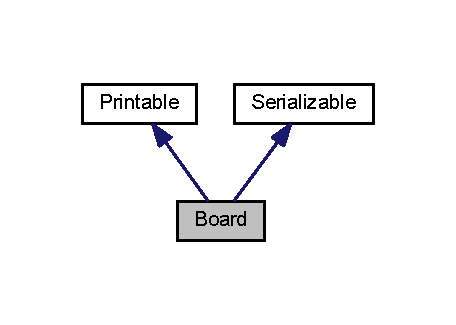
\includegraphics[width=219pt]{class_board__inherit__graph}
\end{center}
\end{figure}


Collaboration diagram for Board\-:
\nopagebreak
\begin{figure}[H]
\begin{center}
\leavevmode
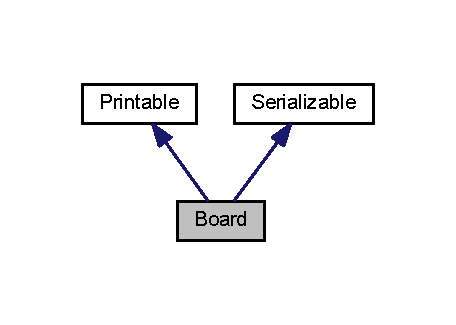
\includegraphics[width=219pt]{class_board__coll__graph}
\end{center}
\end{figure}
\subsection*{Public Types}
\begin{DoxyCompactItemize}
\item 
enum \hyperlink{class_board_a7a90fdd0f301fc502684108416605644}{Type} \{ {\bfseries H\-N\-E\-F\-A\-T\-A\-F\-L}, 
{\bfseries A\-L\-E\-A}, 
{\bfseries T\-A\-B\-L\-U\-T}
 \}
\begin{DoxyCompactList}\small\item\em Different types of boards. \end{DoxyCompactList}\end{DoxyCompactItemize}
\subsection*{Public Member Functions}
\begin{DoxyCompactItemize}
\item 
\hyperlink{class_board_a469583fc5c99cd2aa4c6b6bd1250743b}{Board} (void)
\begin{DoxyCompactList}\small\item\em Default \hyperlink{class_board}{Board} constructor. \end{DoxyCompactList}\item 
\hypertarget{class_board_a0830880c4f04fa4500e23d67dfec525d}{\hyperlink{class_board_a0830880c4f04fa4500e23d67dfec525d}{Board} (const \hyperlink{class_board}{Board} \&src)}\label{class_board_a0830880c4f04fa4500e23d67dfec525d}

\begin{DoxyCompactList}\small\item\em Copy \hyperlink{class_board}{Board} constructor. \end{DoxyCompactList}\item 
\hyperlink{class_board_af67811d3be762bf75ebe5b2dc4b3070e}{Board} (const \hyperlink{class_board_a7a90fdd0f301fc502684108416605644}{Board\-::\-Type} \hyperlink{class_board_a05a3dd8f1f000e20e743e894163228ec}{type}=Board\-::\-Type\-::\-H\-N\-E\-F\-A\-T\-A\-F\-L)
\begin{DoxyCompactList}\small\item\em \hyperlink{class_board}{Board} constructor with setting of boardtype. \end{DoxyCompactList}\item 
\hypertarget{class_board_a737c0ecdabeccd0460bcbae2f8ac6c44}{\hyperlink{class_board_a737c0ecdabeccd0460bcbae2f8ac6c44}{$\sim$\-Board} (void)}\label{class_board_a737c0ecdabeccd0460bcbae2f8ac6c44}

\begin{DoxyCompactList}\small\item\em \hyperlink{class_board}{Board} destructor. \end{DoxyCompactList}\item 
\hyperlink{class_board}{Board} \& \hyperlink{class_board_a57a4317cebaae4f6879856262cf9caae}{operator=} (const \hyperlink{class_board}{Board} \&rhs)
\begin{DoxyCompactList}\small\item\em \hyperlink{class_board}{Board} assignment operator. \end{DoxyCompactList}\item 
\hyperlink{class_tile}{Tile} $\ast$ \hyperlink{class_board_a4dd030ffcb9abc165ace3734e34dd26f}{get\-Tile} (sf\-::\-Vector2$<$ int $>$ pos)
\begin{DoxyCompactList}\small\item\em Returns a pointer to the tile at position pos. \end{DoxyCompactList}\item 
\hypertarget{class_board_a7cef7a9ca499d64c71cb170d67f76ad0}{void \hyperlink{class_board_a7cef7a9ca499d64c71cb170d67f76ad0}{reset\-Board} ()}\label{class_board_a7cef7a9ca499d64c71cb170d67f76ad0}

\begin{DoxyCompactList}\small\item\em Resets the board according to \hyperlink{class_board_a7a90fdd0f301fc502684108416605644}{Board\-::\-Type} \-\_\-type. \end{DoxyCompactList}\item 
\hypertarget{class_board_af7b2ac390d5b62212f7b0ba98276e837}{void \hyperlink{class_board_af7b2ac390d5b62212f7b0ba98276e837}{load\-Board} ()}\label{class_board_af7b2ac390d5b62212f7b0ba98276e837}

\begin{DoxyCompactList}\small\item\em Loads piece positions based on current type. \end{DoxyCompactList}\item 
void \hyperlink{class_board_a7954dc515c68c3d8926355b1c80cc05f}{load\-Board} (const std\-::string \&path)
\begin{DoxyCompactList}\small\item\em Loads piece positions from file path. \end{DoxyCompactList}\item 
void \hyperlink{class_board_a67c2acd87290a3359c8244a4cb72b380}{save\-Board} (const std\-::string \&path)
\begin{DoxyCompactList}\small\item\em Saves piece positions to file path. \end{DoxyCompactList}\item 
void \hyperlink{class_board_a05a3dd8f1f000e20e743e894163228ec}{type} (const \hyperlink{class_board_a7a90fdd0f301fc502684108416605644}{Board\-::\-Type} \&type)
\begin{DoxyCompactList}\small\item\em Sets the type of the board. \end{DoxyCompactList}\item 
const \hyperlink{class_board_a7a90fdd0f301fc502684108416605644}{Board\-::\-Type} \& \hyperlink{class_board_ab2574abe1bfa632795d2b35ba1acb2e4}{type} () const 
\begin{DoxyCompactList}\small\item\em Gets the type of the board. \end{DoxyCompactList}\item 
std\-::string \hyperlink{class_board_a2cf2b2f6adc453bc3b086c9f10c77e11}{to\-String} ()
\begin{DoxyCompactList}\small\item\em Gets information about the current piece. \end{DoxyCompactList}\item 
\hypertarget{class_board_a84aaf6583d8b174ef864dc774979b1a2}{const int \& \hyperlink{class_board_a84aaf6583d8b174ef864dc774979b1a2}{size} () const }\label{class_board_a84aaf6583d8b174ef864dc774979b1a2}

\begin{DoxyCompactList}\small\item\em Returns the boards size. \end{DoxyCompactList}\item 
\hypertarget{class_board_ab0459595994fae0457f0cf58cd6096a1}{void \hyperlink{class_board_ab0459595994fae0457f0cf58cd6096a1}{serialize} (Json\-::\-Value \&root)}\label{class_board_ab0459595994fae0457f0cf58cd6096a1}

\begin{DoxyCompactList}\small\item\em Serialize the object to J\-S\-O\-N. \end{DoxyCompactList}\item 
\hypertarget{class_board_a40f5300d8b4d641d3123a6e9c3a49a45}{void \hyperlink{class_board_a40f5300d8b4d641d3123a6e9c3a49a45}{de\-Serialize} (Json\-::\-Value \&root)}\label{class_board_a40f5300d8b4d641d3123a6e9c3a49a45}

\begin{DoxyCompactList}\small\item\em Deserialize the object. \end{DoxyCompactList}\end{DoxyCompactItemize}


\subsection{Detailed Description}
Defines a board for Hnefatafl. 

\begin{DoxyAuthor}{Author}
Rasmus Pettersson Vik 
\end{DoxyAuthor}
\begin{DoxyDate}{Date}
juni 2013 
\end{DoxyDate}


\subsection{Constructor \& Destructor Documentation}
\hypertarget{class_board_a469583fc5c99cd2aa4c6b6bd1250743b}{\index{Board@{Board}!Board@{Board}}
\index{Board@{Board}!Board@{Board}}
\subsubsection[{Board}]{\setlength{\rightskip}{0pt plus 5cm}Board\-::\-Board (
\begin{DoxyParamCaption}
\item[{void}]{}
\end{DoxyParamCaption}
)}}\label{class_board_a469583fc5c99cd2aa4c6b6bd1250743b}


Default \hyperlink{class_board}{Board} constructor. 

Initialises board object with type of Board\-::\-Type\-::\-H\-N\-E\-F\-A\-T\-A\-F\-L and adds tiles to the tiles vector. \hyperlink{class_board}{Board} will be 11x11. Loads starting positions from starting\-Pos/hnefatafl.\-txt and adds pieces. 

Here is the call graph for this function\-:\nopagebreak
\begin{figure}[H]
\begin{center}
\leavevmode
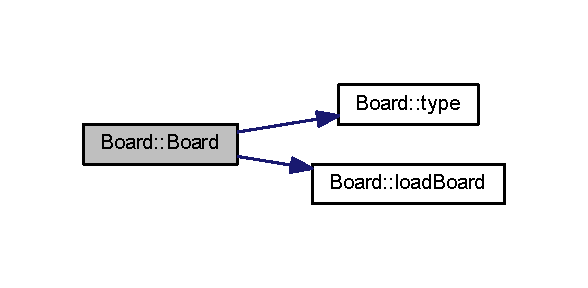
\includegraphics[width=282pt]{class_board_a469583fc5c99cd2aa4c6b6bd1250743b_cgraph}
\end{center}
\end{figure}


\hypertarget{class_board_af67811d3be762bf75ebe5b2dc4b3070e}{\index{Board@{Board}!Board@{Board}}
\index{Board@{Board}!Board@{Board}}
\subsubsection[{Board}]{\setlength{\rightskip}{0pt plus 5cm}Board\-::\-Board (
\begin{DoxyParamCaption}
\item[{const {\bf Board\-::\-Type}}]{type = {\ttfamily Board\-:\-:Type\-:\-:HNEFATAFL}}
\end{DoxyParamCaption}
)}}\label{class_board_af67811d3be762bf75ebe5b2dc4b3070e}


\hyperlink{class_board}{Board} constructor with setting of boardtype. 

Initialises board object with type of \hyperlink{class_board_a7a90fdd0f301fc502684108416605644}{Board\-::\-Type} and loads corresponding starting positions and adds tiles and pieces. 

Here is the call graph for this function\-:\nopagebreak
\begin{figure}[H]
\begin{center}
\leavevmode
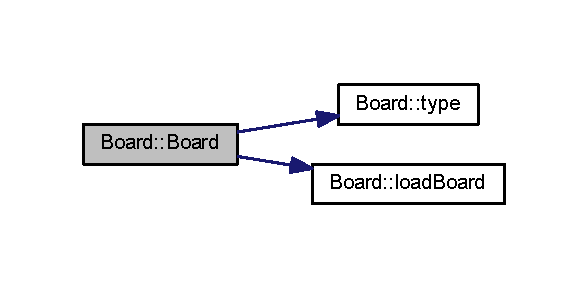
\includegraphics[width=282pt]{class_board_af67811d3be762bf75ebe5b2dc4b3070e_cgraph}
\end{center}
\end{figure}




\subsection{Member Function Documentation}
\hypertarget{class_board_a4dd030ffcb9abc165ace3734e34dd26f}{\index{Board@{Board}!get\-Tile@{get\-Tile}}
\index{get\-Tile@{get\-Tile}!Board@{Board}}
\subsubsection[{get\-Tile}]{\setlength{\rightskip}{0pt plus 5cm}{\bf Tile}$\ast$ Board\-::get\-Tile (
\begin{DoxyParamCaption}
\item[{sf\-::\-Vector2$<$ int $>$}]{pos}
\end{DoxyParamCaption}
)}}\label{class_board_a4dd030ffcb9abc165ace3734e34dd26f}


Returns a pointer to the tile at position pos. 


\begin{DoxyParams}[1]{Parameters}
\mbox{\tt in}  & {\em pos} & Position to tile on board. \\
\hline
\end{DoxyParams}
\begin{DoxyReturn}{Returns}
Returns a pointer to the tile at given position. If pos is less than 0 or greater than \hyperlink{class_board_a84aaf6583d8b174ef864dc774979b1a2}{Board.\-size()} function returns nullptr. 
\end{DoxyReturn}
\hypertarget{class_board_a7954dc515c68c3d8926355b1c80cc05f}{\index{Board@{Board}!load\-Board@{load\-Board}}
\index{load\-Board@{load\-Board}!Board@{Board}}
\subsubsection[{load\-Board}]{\setlength{\rightskip}{0pt plus 5cm}void Board\-::load\-Board (
\begin{DoxyParamCaption}
\item[{const std\-::string \&}]{path}
\end{DoxyParamCaption}
)}}\label{class_board_a7954dc515c68c3d8926355b1c80cc05f}


Loads piece positions from file path. 


\begin{DoxyParams}[1]{Parameters}
\mbox{\tt in}  & {\em path} & File to load positions from. \\
\hline
\end{DoxyParams}
\hypertarget{class_board_a57a4317cebaae4f6879856262cf9caae}{\index{Board@{Board}!operator=@{operator=}}
\index{operator=@{operator=}!Board@{Board}}
\subsubsection[{operator=}]{\setlength{\rightskip}{0pt plus 5cm}{\bf Board} \& Board\-::operator= (
\begin{DoxyParamCaption}
\item[{const {\bf Board} \&}]{rhs}
\end{DoxyParamCaption}
)}}\label{class_board_a57a4317cebaae4f6879856262cf9caae}


\hyperlink{class_board}{Board} assignment operator. 


\begin{DoxyParams}[1]{Parameters}
\mbox{\tt in}  & {\em rhs} & Source to copy from \\
\hline
\end{DoxyParams}
\hypertarget{class_board_a67c2acd87290a3359c8244a4cb72b380}{\index{Board@{Board}!save\-Board@{save\-Board}}
\index{save\-Board@{save\-Board}!Board@{Board}}
\subsubsection[{save\-Board}]{\setlength{\rightskip}{0pt plus 5cm}void Board\-::save\-Board (
\begin{DoxyParamCaption}
\item[{const std\-::string \&}]{path}
\end{DoxyParamCaption}
)}}\label{class_board_a67c2acd87290a3359c8244a4cb72b380}


Saves piece positions to file path. 


\begin{DoxyParams}[1]{Parameters}
\mbox{\tt in}  & {\em path} & File to save positions to. \\
\hline
\end{DoxyParams}
\hypertarget{class_board_a2cf2b2f6adc453bc3b086c9f10c77e11}{\index{Board@{Board}!to\-String@{to\-String}}
\index{to\-String@{to\-String}!Board@{Board}}
\subsubsection[{to\-String}]{\setlength{\rightskip}{0pt plus 5cm}std\-::string Board\-::to\-String (
\begin{DoxyParamCaption}
{}
\end{DoxyParamCaption}
)\hspace{0.3cm}{\ttfamily [virtual]}}}\label{class_board_a2cf2b2f6adc453bc3b086c9f10c77e11}


Gets information about the current piece. 

\begin{DoxyReturn}{Returns}
Returns the type and position of the piece in a human readable format. 
\end{DoxyReturn}


Implements \hyperlink{class_printable_a489f74384330f76d048d1ccf5c541571}{Printable}.

\hypertarget{class_board_a05a3dd8f1f000e20e743e894163228ec}{\index{Board@{Board}!type@{type}}
\index{type@{type}!Board@{Board}}
\subsubsection[{type}]{\setlength{\rightskip}{0pt plus 5cm}void Board\-::type (
\begin{DoxyParamCaption}
\item[{const {\bf Board\-::\-Type} \&}]{type}
\end{DoxyParamCaption}
)}}\label{class_board_a05a3dd8f1f000e20e743e894163228ec}


Sets the type of the board. 


\begin{DoxyParams}[1]{Parameters}
\mbox{\tt in}  & {\em type} & The type of the board \\
\hline
\end{DoxyParams}


Here is the call graph for this function\-:\nopagebreak
\begin{figure}[H]
\begin{center}
\leavevmode
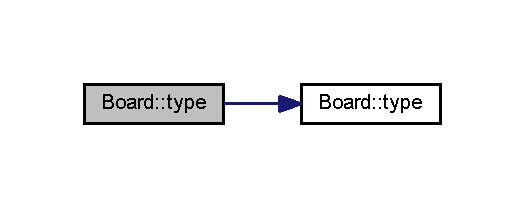
\includegraphics[width=252pt]{class_board_a05a3dd8f1f000e20e743e894163228ec_cgraph}
\end{center}
\end{figure}


\hypertarget{class_board_ab2574abe1bfa632795d2b35ba1acb2e4}{\index{Board@{Board}!type@{type}}
\index{type@{type}!Board@{Board}}
\subsubsection[{type}]{\setlength{\rightskip}{0pt plus 5cm}const {\bf Board\-::\-Type} \& Board\-::type (
\begin{DoxyParamCaption}
{}
\end{DoxyParamCaption}
) const}}\label{class_board_ab2574abe1bfa632795d2b35ba1acb2e4}


Gets the type of the board. 

\begin{DoxyReturn}{Returns}
Returns the type of the board 
\end{DoxyReturn}


Here is the caller graph for this function\-:\nopagebreak
\begin{figure}[H]
\begin{center}
\leavevmode
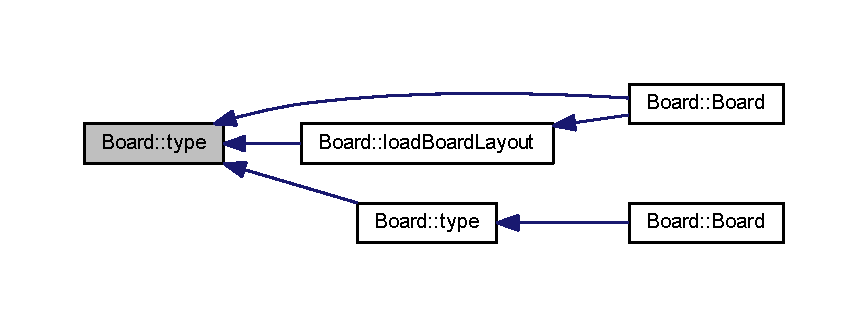
\includegraphics[width=258pt]{class_board_ab2574abe1bfa632795d2b35ba1acb2e4_icgraph}
\end{center}
\end{figure}




The documentation for this class was generated from the following files\-:\begin{DoxyCompactItemize}
\item 
Hnefatafl/\hyperlink{_board_8hpp}{Board.\-hpp}\item 
Hnefatafl/Board.\-cpp\end{DoxyCompactItemize}

\hypertarget{class_board_entity}{\section{Board\-Entity Class Reference}
\label{class_board_entity}\index{Board\-Entity@{Board\-Entity}}
}


Abstract baseclass for an entity with a position on the gameboard.  




{\ttfamily \#include $<$Board\-Entity.\-hpp$>$}



Inheritance diagram for Board\-Entity\-:\nopagebreak
\begin{figure}[H]
\begin{center}
\leavevmode
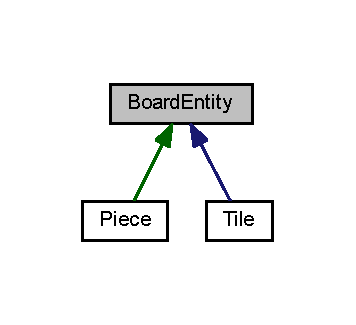
\includegraphics[width=171pt]{class_board_entity__inherit__graph}
\end{center}
\end{figure}
\subsection*{Public Member Functions}
\begin{DoxyCompactItemize}
\item 
\hypertarget{class_board_entity_a809e46488b5db0ca8940176296548d4c}{\hyperlink{class_board_entity_a809e46488b5db0ca8940176296548d4c}{Board\-Entity} (void)}\label{class_board_entity_a809e46488b5db0ca8940176296548d4c}

\begin{DoxyCompactList}\small\item\em Default \hyperlink{class_board_entity}{Board\-Entity} Constructor Runs \hyperlink{class_board_entity_abb7251fa8167ce5618076a79427c8521}{\-\_\-init()} and initialises \-\_\-position to (-\/1, -\/1) \end{DoxyCompactList}\item 
\hypertarget{class_board_entity_a5856127ebd5b45c32e745cca13b0775d}{virtual \hyperlink{class_board_entity_a5856127ebd5b45c32e745cca13b0775d}{$\sim$\-Board\-Entity} (void)}\label{class_board_entity_a5856127ebd5b45c32e745cca13b0775d}

\begin{DoxyCompactList}\small\item\em Virtual \hyperlink{class_board_entity}{Board\-Entity} destructor. \end{DoxyCompactList}\item 
void \hyperlink{class_board_entity_a177b0ebff2150101415eb70b4fc677cb}{position} (const sf\-::\-Vector2$<$ int $>$ \&pos)
\begin{DoxyCompactList}\small\item\em Sets the position of the \hyperlink{class_board_entity}{Board\-Entity}. \end{DoxyCompactList}\item 
const sf\-::\-Vector2$<$ int $>$ \& \hyperlink{class_board_entity_aef7592bf7ad04fb47402cbbea5fac723}{position} () const 
\begin{DoxyCompactList}\small\item\em Gets the position of the \hyperlink{class_board_entity}{Board\-Entity}. \end{DoxyCompactList}\end{DoxyCompactItemize}
\subsection*{Protected Member Functions}
\begin{DoxyCompactItemize}
\item 
virtual void \hyperlink{class_board_entity_abb7251fa8167ce5618076a79427c8521}{\-\_\-init} ()=0
\end{DoxyCompactItemize}
\subsection*{Protected Attributes}
\begin{DoxyCompactItemize}
\item 
\hypertarget{class_board_entity_a2c4f3a3dbd1aa78abc228ce86d109303}{sf\-::\-Vector2$<$ int $>$ \hyperlink{class_board_entity_a2c4f3a3dbd1aa78abc228ce86d109303}{\-\_\-position}}\label{class_board_entity_a2c4f3a3dbd1aa78abc228ce86d109303}

\begin{DoxyCompactList}\small\item\em Holds the current position of the \hyperlink{class_board_entity}{Board\-Entity}. \end{DoxyCompactList}\end{DoxyCompactItemize}


\subsection{Detailed Description}
Abstract baseclass for an entity with a position on the gameboard. 

\begin{DoxyAuthor}{Author}
Rasmus Pettersson Vik 
\end{DoxyAuthor}
\begin{DoxyDate}{Date}
juni 2013 
\end{DoxyDate}


\subsection{Member Function Documentation}
\hypertarget{class_board_entity_abb7251fa8167ce5618076a79427c8521}{\index{Board\-Entity@{Board\-Entity}!\-\_\-init@{\-\_\-init}}
\index{\-\_\-init@{\-\_\-init}!BoardEntity@{Board\-Entity}}
\subsubsection[{\-\_\-init}]{\setlength{\rightskip}{0pt plus 5cm}void Board\-Entity\-::\-\_\-init (
\begin{DoxyParamCaption}
{}
\end{DoxyParamCaption}
)\hspace{0.3cm}{\ttfamily [protected]}, {\ttfamily [pure virtual]}}}\label{class_board_entity_abb7251fa8167ce5618076a79427c8521}
Initialising function \begin{DoxyNote}{Note}
Should be run in every constructor! 
\end{DoxyNote}


Here is the caller graph for this function\-:\nopagebreak
\begin{figure}[H]
\begin{center}
\leavevmode
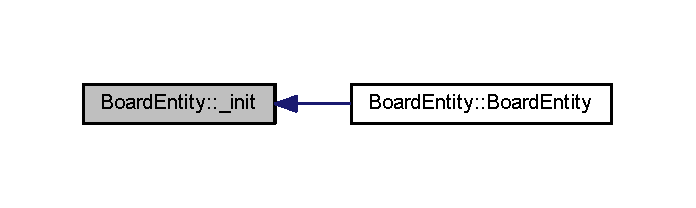
\includegraphics[width=334pt]{class_board_entity_abb7251fa8167ce5618076a79427c8521_icgraph}
\end{center}
\end{figure}


\hypertarget{class_board_entity_a177b0ebff2150101415eb70b4fc677cb}{\index{Board\-Entity@{Board\-Entity}!position@{position}}
\index{position@{position}!BoardEntity@{Board\-Entity}}
\subsubsection[{position}]{\setlength{\rightskip}{0pt plus 5cm}void Board\-Entity\-::position (
\begin{DoxyParamCaption}
\item[{const sf\-::\-Vector2$<$ int $>$ \&}]{pos}
\end{DoxyParamCaption}
)}}\label{class_board_entity_a177b0ebff2150101415eb70b4fc677cb}


Sets the position of the \hyperlink{class_board_entity}{Board\-Entity}. 


\begin{DoxyParams}[1]{Parameters}
\mbox{\tt in}  & {\em pos} & The position to set. \\
\hline
\end{DoxyParams}


Here is the caller graph for this function\-:\nopagebreak
\begin{figure}[H]
\begin{center}
\leavevmode
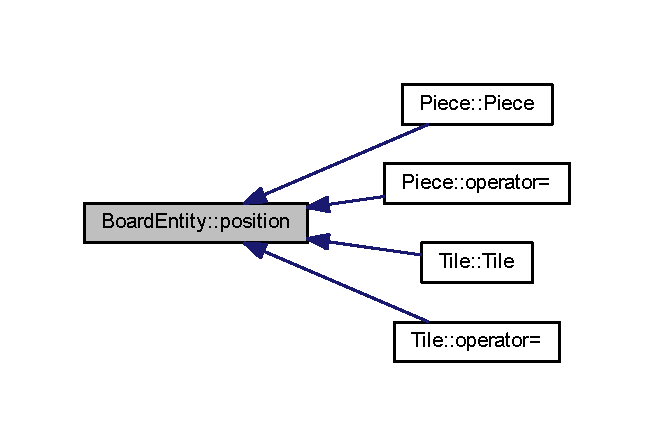
\includegraphics[width=296pt]{class_board_entity_a177b0ebff2150101415eb70b4fc677cb_icgraph}
\end{center}
\end{figure}


\hypertarget{class_board_entity_aef7592bf7ad04fb47402cbbea5fac723}{\index{Board\-Entity@{Board\-Entity}!position@{position}}
\index{position@{position}!BoardEntity@{Board\-Entity}}
\subsubsection[{position}]{\setlength{\rightskip}{0pt plus 5cm}const sf\-::\-Vector2$<$ int $>$ \& Board\-Entity\-::position (
\begin{DoxyParamCaption}
{}
\end{DoxyParamCaption}
) const}}\label{class_board_entity_aef7592bf7ad04fb47402cbbea5fac723}


Gets the position of the \hyperlink{class_board_entity}{Board\-Entity}. 

\begin{DoxyReturn}{Returns}
Gets the position of the \hyperlink{class_board_entity}{Board\-Entity}. 
\end{DoxyReturn}


Here is the caller graph for this function\-:\nopagebreak
\begin{figure}[H]
\begin{center}
\leavevmode
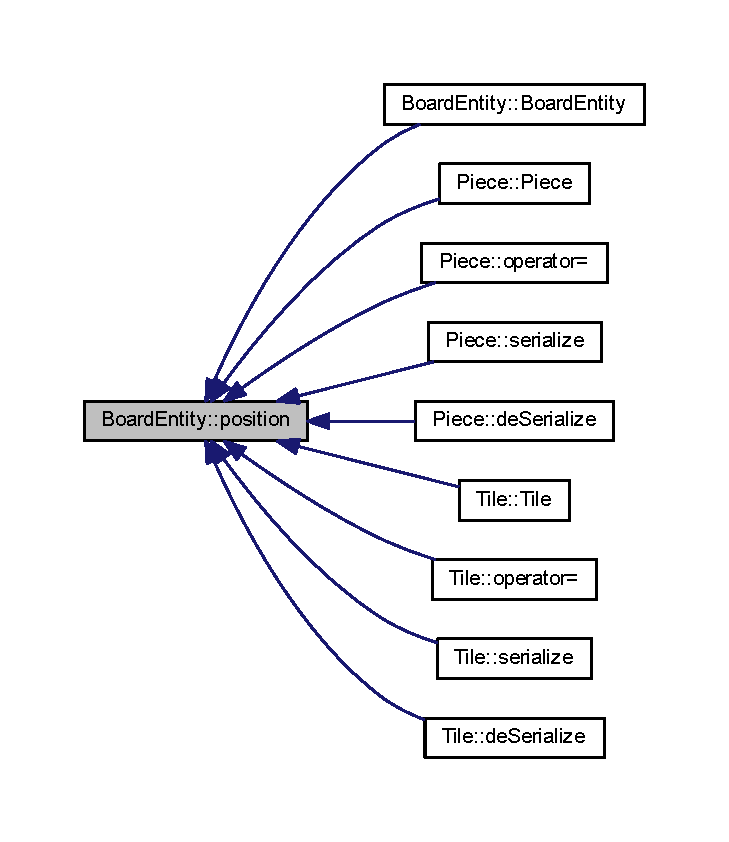
\includegraphics[width=350pt]{class_board_entity_aef7592bf7ad04fb47402cbbea5fac723_icgraph}
\end{center}
\end{figure}




The documentation for this class was generated from the following files\-:\begin{DoxyCompactItemize}
\item 
D\-:/git ws/\-Hnefatafl/\-Hnefatafl/\hyperlink{_board_entity_8hpp}{Board\-Entity.\-hpp}\item 
D\-:/git ws/\-Hnefatafl/\-Hnefatafl/\hyperlink{_board_entity_8cpp}{Board\-Entity.\-cpp}\end{DoxyCompactItemize}

\hypertarget{class_piece}{\section{Piece Class Reference}
\label{class_piece}\index{Piece@{Piece}}
}


Describes a piece on the gameboard.  




{\ttfamily \#include $<$Piece.\-hpp$>$}



Inheritance diagram for Piece\-:
\nopagebreak
\begin{figure}[H]
\begin{center}
\leavevmode
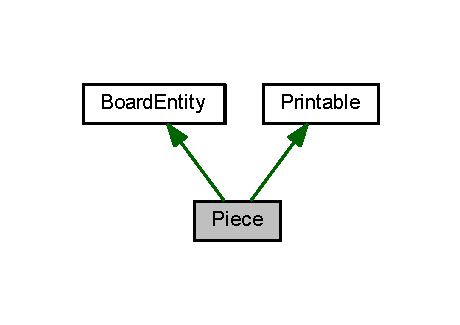
\includegraphics[width=306pt]{class_piece__inherit__graph}
\end{center}
\end{figure}


Collaboration diagram for Piece\-:
\nopagebreak
\begin{figure}[H]
\begin{center}
\leavevmode
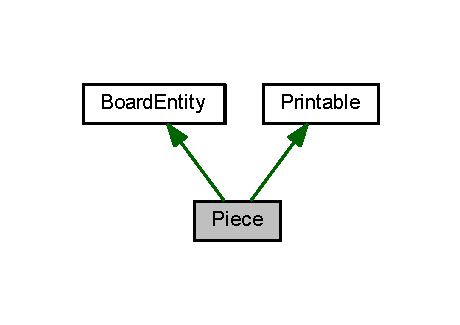
\includegraphics[width=306pt]{class_piece__coll__graph}
\end{center}
\end{figure}
\subsection*{Public Types}
\begin{DoxyCompactItemize}
\item 
enum \hyperlink{class_piece_abcd044975b3657962abfd2ded9194b09}{Type} \{ {\bfseries B\-L\-A\-C\-K}, 
{\bfseries W\-H\-I\-T\-E}, 
{\bfseries K\-I\-N\-G}
 \}
\begin{DoxyCompactList}\small\item\em Different types of Pieces. \end{DoxyCompactList}\end{DoxyCompactItemize}
\subsection*{Public Member Functions}
\begin{DoxyCompactItemize}
\item 
\hypertarget{class_piece_a64870ec3fe38b7f88c802d91db861abb}{\hyperlink{class_piece_a64870ec3fe38b7f88c802d91db861abb}{Piece} (void)}\label{class_piece_a64870ec3fe38b7f88c802d91db861abb}

\begin{DoxyCompactList}\small\item\em Default \hyperlink{class_piece}{Piece} Constructor Initialises tile object with Piece\-::\-Type\-::\-Black and position -\/1, -\/1. \end{DoxyCompactList}\item 
\hyperlink{class_piece_a97dfab7bb313f6e94eb23d4b8736bdac}{Piece} (const \hyperlink{class_piece}{Piece} \&src)
\begin{DoxyCompactList}\small\item\em \hyperlink{class_piece}{Piece} copy constructor. \end{DoxyCompactList}\item 
\hyperlink{class_piece_a0602222d442db964778b25d3e7b930cc}{Piece} (const sf\-::\-Vector2$<$ int $>$ \&pos, const \hyperlink{class_piece_abcd044975b3657962abfd2ded9194b09}{Piece\-::\-Type} \&\hyperlink{class_piece_ad41386c09d8ca34799398a2c11036cce}{type}=Piece\-::\-Type\-::\-B\-L\-A\-C\-K)
\begin{DoxyCompactList}\small\item\em \hyperlink{class_piece}{Piece} constructor with position and type. \end{DoxyCompactList}\item 
\hypertarget{class_piece_ad28316e726ffa96f258a79ea90e41d16}{\hyperlink{class_piece_ad28316e726ffa96f258a79ea90e41d16}{$\sim$\-Piece} (void)}\label{class_piece_ad28316e726ffa96f258a79ea90e41d16}

\begin{DoxyCompactList}\small\item\em \hyperlink{class_piece}{Piece} destructor. \end{DoxyCompactList}\item 
\hyperlink{class_piece}{Piece} \& \hyperlink{class_piece_a8b059420684d0bf0ed7cde80b42a6286}{operator=} (const \hyperlink{class_piece}{Piece} \&rhs)
\begin{DoxyCompactList}\small\item\em \hyperlink{class_piece}{Piece} assignment operator. \end{DoxyCompactList}\item 
void \hyperlink{class_piece_ad41386c09d8ca34799398a2c11036cce}{type} (const \hyperlink{class_piece_abcd044975b3657962abfd2ded9194b09}{Piece\-::\-Type} \&type)
\begin{DoxyCompactList}\small\item\em Sets the type of the piece. \end{DoxyCompactList}\item 
const \hyperlink{class_piece_abcd044975b3657962abfd2ded9194b09}{Piece\-::\-Type} \& \hyperlink{class_piece_a64d970cf7c3d34014d8a36cc3bd3c908}{type} () const 
\begin{DoxyCompactList}\small\item\em Gets the type of the piece. \end{DoxyCompactList}\item 
std\-::string \hyperlink{class_piece_ae18523c400cb72a50bb1293d27cd1432}{to\-String} ()
\begin{DoxyCompactList}\small\item\em Gets information about the current piece. \end{DoxyCompactList}\item 
\hypertarget{class_piece_ae2397428f87d0303ede94fa91fef5ea5}{void \hyperlink{class_piece_ae2397428f87d0303ede94fa91fef5ea5}{serialize} (Json\-::\-Value \&root)}\label{class_piece_ae2397428f87d0303ede94fa91fef5ea5}

\begin{DoxyCompactList}\small\item\em Serialize the object to J\-S\-O\-N. \end{DoxyCompactList}\item 
\hypertarget{class_piece_a51f5d80dc3584e372d356ebfc281a886}{void \hyperlink{class_piece_a51f5d80dc3584e372d356ebfc281a886}{de\-Serialize} (Json\-::\-Value \&root)}\label{class_piece_a51f5d80dc3584e372d356ebfc281a886}

\begin{DoxyCompactList}\small\item\em Deserialize the object. \end{DoxyCompactList}\end{DoxyCompactItemize}
\subsection*{Additional Inherited Members}


\subsection{Detailed Description}
Describes a piece on the gameboard. 

\begin{DoxyAuthor}{Author}
Rasmus Pettersson Vik 
\end{DoxyAuthor}
\begin{DoxyDate}{Date}
juni 2013 
\end{DoxyDate}


\subsection{Constructor \& Destructor Documentation}
\hypertarget{class_piece_a97dfab7bb313f6e94eb23d4b8736bdac}{\index{Piece@{Piece}!Piece@{Piece}}
\index{Piece@{Piece}!Piece@{Piece}}
\subsubsection[{Piece}]{\setlength{\rightskip}{0pt plus 5cm}Piece\-::\-Piece (
\begin{DoxyParamCaption}
\item[{const {\bf Piece} \&}]{src}
\end{DoxyParamCaption}
)}}\label{class_piece_a97dfab7bb313f6e94eb23d4b8736bdac}


\hyperlink{class_piece}{Piece} copy constructor. 


\begin{DoxyParams}[1]{Parameters}
\mbox{\tt in}  & {\em src} & Source to copy from \\
\hline
\end{DoxyParams}


Here is the call graph for this function\-:\nopagebreak
\begin{figure}[H]
\begin{center}
\leavevmode
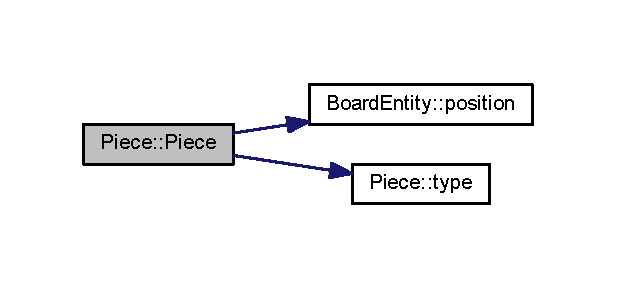
\includegraphics[width=296pt]{class_piece_a97dfab7bb313f6e94eb23d4b8736bdac_cgraph}
\end{center}
\end{figure}


\hypertarget{class_piece_a0602222d442db964778b25d3e7b930cc}{\index{Piece@{Piece}!Piece@{Piece}}
\index{Piece@{Piece}!Piece@{Piece}}
\subsubsection[{Piece}]{\setlength{\rightskip}{0pt plus 5cm}Piece\-::\-Piece (
\begin{DoxyParamCaption}
\item[{const sf\-::\-Vector2$<$ int $>$ \&}]{pos, }
\item[{const {\bf Piece\-::\-Type} \&}]{type = {\ttfamily Piece\-:\-:Type\-:\-:BLACK}}
\end{DoxyParamCaption}
)}}\label{class_piece_a0602222d442db964778b25d3e7b930cc}


\hyperlink{class_piece}{Piece} constructor with position and type. 

Initializes tile object with the position pos and default type of Piece\-::\-Type\-::\-B\-L\-A\-C\-K.


\begin{DoxyParams}[1]{Parameters}
\mbox{\tt in}  & {\em pos} & The position to set the piece to. \\
\hline
\mbox{\tt in}  & {\em type} & The type to set the piece to. Default is Piece\-::\-Type\-::\-B\-L\-A\-C\-K. \\
\hline
\end{DoxyParams}


Here is the call graph for this function\-:\nopagebreak
\begin{figure}[H]
\begin{center}
\leavevmode
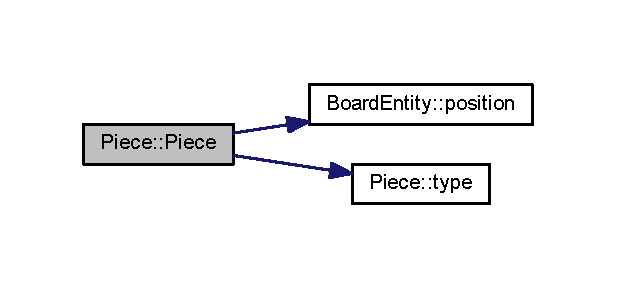
\includegraphics[width=296pt]{class_piece_a0602222d442db964778b25d3e7b930cc_cgraph}
\end{center}
\end{figure}




\subsection{Member Function Documentation}
\hypertarget{class_piece_a8b059420684d0bf0ed7cde80b42a6286}{\index{Piece@{Piece}!operator=@{operator=}}
\index{operator=@{operator=}!Piece@{Piece}}
\subsubsection[{operator=}]{\setlength{\rightskip}{0pt plus 5cm}{\bf Piece} \& Piece\-::operator= (
\begin{DoxyParamCaption}
\item[{const {\bf Piece} \&}]{rhs}
\end{DoxyParamCaption}
)}}\label{class_piece_a8b059420684d0bf0ed7cde80b42a6286}


\hyperlink{class_piece}{Piece} assignment operator. 


\begin{DoxyParams}[1]{Parameters}
\mbox{\tt in}  & {\em rhs} & Source to copy from \\
\hline
\end{DoxyParams}


Here is the call graph for this function\-:\nopagebreak
\begin{figure}[H]
\begin{center}
\leavevmode
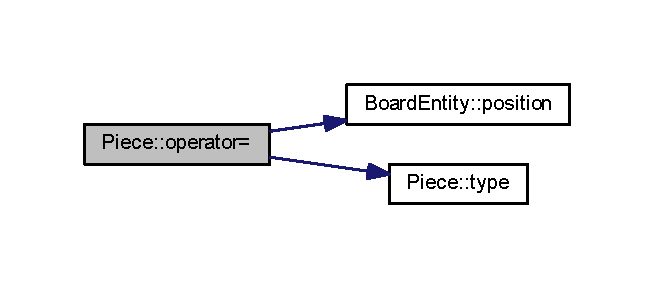
\includegraphics[width=314pt]{class_piece_a8b059420684d0bf0ed7cde80b42a6286_cgraph}
\end{center}
\end{figure}


\hypertarget{class_piece_ae18523c400cb72a50bb1293d27cd1432}{\index{Piece@{Piece}!to\-String@{to\-String}}
\index{to\-String@{to\-String}!Piece@{Piece}}
\subsubsection[{to\-String}]{\setlength{\rightskip}{0pt plus 5cm}std\-::string Piece\-::to\-String (
\begin{DoxyParamCaption}
{}
\end{DoxyParamCaption}
)\hspace{0.3cm}{\ttfamily [virtual]}}}\label{class_piece_ae18523c400cb72a50bb1293d27cd1432}


Gets information about the current piece. 

\begin{DoxyReturn}{Returns}
Returns the type and position of the piece in a human readable format. 
\end{DoxyReturn}


Implements \hyperlink{class_printable_a489f74384330f76d048d1ccf5c541571}{Printable}.

\hypertarget{class_piece_ad41386c09d8ca34799398a2c11036cce}{\index{Piece@{Piece}!type@{type}}
\index{type@{type}!Piece@{Piece}}
\subsubsection[{type}]{\setlength{\rightskip}{0pt plus 5cm}void Piece\-::type (
\begin{DoxyParamCaption}
\item[{const {\bf Piece\-::\-Type} \&}]{type}
\end{DoxyParamCaption}
)}}\label{class_piece_ad41386c09d8ca34799398a2c11036cce}


Sets the type of the piece. 


\begin{DoxyParams}[1]{Parameters}
\mbox{\tt in}  & {\em type} & The type of the piece \\
\hline
\end{DoxyParams}


Here is the call graph for this function\-:\nopagebreak
\begin{figure}[H]
\begin{center}
\leavevmode
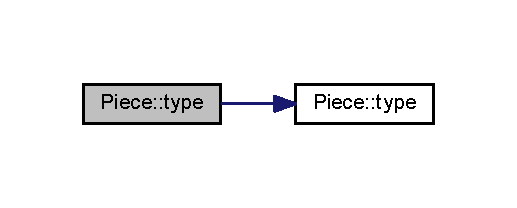
\includegraphics[width=248pt]{class_piece_ad41386c09d8ca34799398a2c11036cce_cgraph}
\end{center}
\end{figure}




Here is the caller graph for this function\-:\nopagebreak
\begin{figure}[H]
\begin{center}
\leavevmode
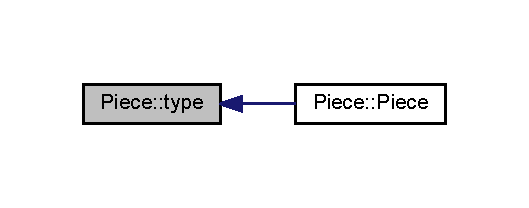
\includegraphics[width=272pt]{class_piece_ad41386c09d8ca34799398a2c11036cce_icgraph}
\end{center}
\end{figure}


\hypertarget{class_piece_a64d970cf7c3d34014d8a36cc3bd3c908}{\index{Piece@{Piece}!type@{type}}
\index{type@{type}!Piece@{Piece}}
\subsubsection[{type}]{\setlength{\rightskip}{0pt plus 5cm}const {\bf Piece\-::\-Type} \& Piece\-::type (
\begin{DoxyParamCaption}
{}
\end{DoxyParamCaption}
) const}}\label{class_piece_a64d970cf7c3d34014d8a36cc3bd3c908}


Gets the type of the piece. 

\begin{DoxyReturn}{Returns}
Returns the type of the piece 
\end{DoxyReturn}


Here is the caller graph for this function\-:
\nopagebreak
\begin{figure}[H]
\begin{center}
\leavevmode
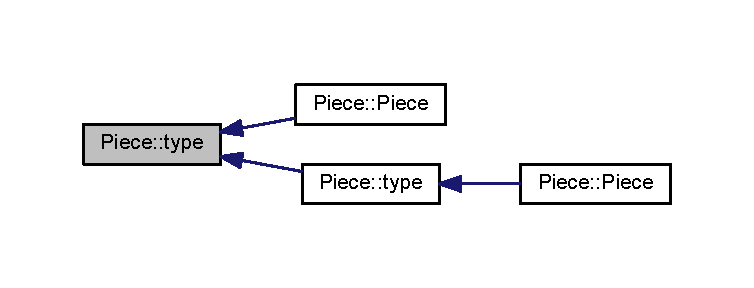
\includegraphics[width=350pt]{class_piece_a64d970cf7c3d34014d8a36cc3bd3c908_icgraph}
\end{center}
\end{figure}




The documentation for this class was generated from the following files\-:\begin{DoxyCompactItemize}
\item 
Hnefatafl/\hyperlink{_piece_8hpp}{Piece.\-hpp}\item 
Hnefatafl/\hyperlink{_piece_8cpp}{Piece.\-cpp}\end{DoxyCompactItemize}

\hypertarget{class_printable}{\section{Printable Class Reference}
\label{class_printable}\index{Printable@{Printable}}
}


Abstract class implementing std\-::string \hyperlink{class_printable_a489f74384330f76d048d1ccf5c541571}{to\-String()} functionality.  




{\ttfamily \#include $<$Printable.\-hpp$>$}



Inheritance diagram for Printable\-:\nopagebreak
\begin{figure}[H]
\begin{center}
\leavevmode
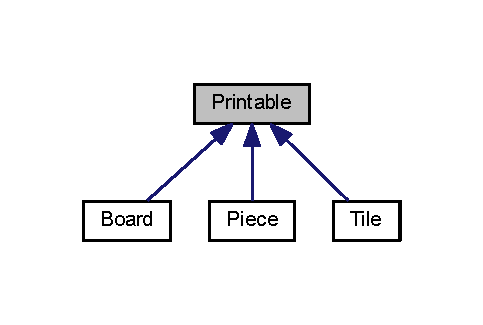
\includegraphics[width=171pt]{class_printable__inherit__graph}
\end{center}
\end{figure}
\subsection*{Public Member Functions}
\begin{DoxyCompactItemize}
\item 
\hypertarget{class_printable_a489f74384330f76d048d1ccf5c541571}{virtual std\-::string \hyperlink{class_printable_a489f74384330f76d048d1ccf5c541571}{to\-String} ()=0}\label{class_printable_a489f74384330f76d048d1ccf5c541571}

\begin{DoxyCompactList}\small\item\em Display information about the object. \end{DoxyCompactList}\end{DoxyCompactItemize}


\subsection{Detailed Description}
Abstract class implementing std\-::string \hyperlink{class_printable_a489f74384330f76d048d1ccf5c541571}{to\-String()} functionality. 

\begin{DoxyAuthor}{Author}
Rasmus Pettersson Vik 
\end{DoxyAuthor}
\begin{DoxyDate}{Date}
juni 2013 
\end{DoxyDate}


The documentation for this class was generated from the following file\-:\begin{DoxyCompactItemize}
\item 
D\-:/git ws/\-Hnefatafl/\-Hnefatafl/\hyperlink{_printable_8hpp}{Printable.\-hpp}\end{DoxyCompactItemize}

\hypertarget{class_serializable}{\section{Serializable Class Reference}
\label{class_serializable}\index{Serializable@{Serializable}}
}


Interface for serializing classes to J\-S\-O\-N.  




{\ttfamily \#include $<$Serializable.\-hpp$>$}



Inheritance diagram for Serializable\-:\nopagebreak
\begin{figure}[H]
\begin{center}
\leavevmode
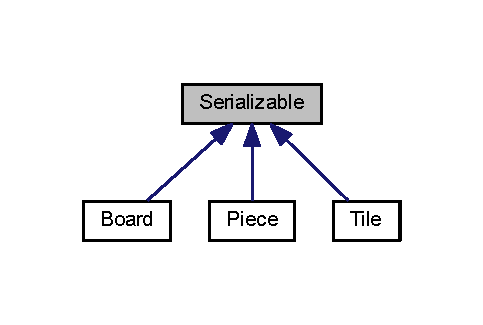
\includegraphics[width=232pt]{class_serializable__inherit__graph}
\end{center}
\end{figure}
\subsection*{Public Member Functions}
\begin{DoxyCompactItemize}
\item 
\hypertarget{class_serializable_a3d7322ec8a0db1573bcabe1590723e31}{virtual \hyperlink{class_serializable_a3d7322ec8a0db1573bcabe1590723e31}{$\sim$\-Serializable} (void)}\label{class_serializable_a3d7322ec8a0db1573bcabe1590723e31}

\begin{DoxyCompactList}\small\item\em Virtual destructor. \end{DoxyCompactList}\item 
virtual void \hyperlink{class_serializable_aa18caa72dd5e441647f86cc7aab62096}{serialize} (Json\-::\-Value \&root)=0
\begin{DoxyCompactList}\small\item\em Pure virtual function to serialize a class. \end{DoxyCompactList}\item 
virtual void \hyperlink{class_serializable_ab423aaa267b7a0c7ad829128acde757c}{de\-Serialize} (Json\-::\-Value \&root)=0
\begin{DoxyCompactList}\small\item\em Pure virtual function to deserialize a class. \end{DoxyCompactList}\end{DoxyCompactItemize}


\subsection{Detailed Description}
Interface for serializing classes to J\-S\-O\-N. 

\begin{DoxyAuthor}{Author}
Rasmus Pettersson Vik 
\end{DoxyAuthor}
\begin{DoxyDate}{Date}
juni 2013 
\end{DoxyDate}


\subsection{Member Function Documentation}
\hypertarget{class_serializable_ab423aaa267b7a0c7ad829128acde757c}{\index{Serializable@{Serializable}!de\-Serialize@{de\-Serialize}}
\index{de\-Serialize@{de\-Serialize}!Serializable@{Serializable}}
\subsubsection[{de\-Serialize}]{\setlength{\rightskip}{0pt plus 5cm}virtual void Serializable\-::de\-Serialize (
\begin{DoxyParamCaption}
\item[{Json\-::\-Value \&}]{root}
\end{DoxyParamCaption}
)\hspace{0.3cm}{\ttfamily [pure virtual]}}}\label{class_serializable_ab423aaa267b7a0c7ad829128acde757c}


Pure virtual function to deserialize a class. 


\begin{DoxyParams}[1]{Parameters}
\mbox{\tt in}  & {\em root} & ... \\
\hline
\end{DoxyParams}


Implemented in \hyperlink{class_board_a40f5300d8b4d641d3123a6e9c3a49a45}{Board}, \hyperlink{class_tile_aac6ff96901aa89ac87b1a8385dc6444d}{Tile}, and \hyperlink{class_piece_a51f5d80dc3584e372d356ebfc281a886}{Piece}.



Here is the caller graph for this function\-:\nopagebreak
\begin{figure}[H]
\begin{center}
\leavevmode
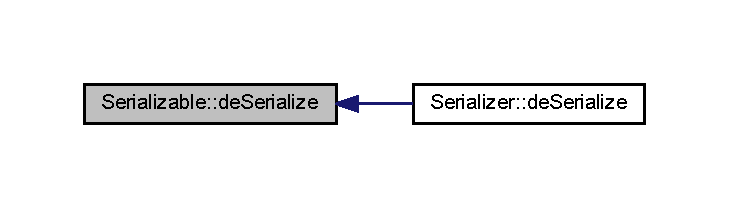
\includegraphics[width=350pt]{class_serializable_ab423aaa267b7a0c7ad829128acde757c_icgraph}
\end{center}
\end{figure}


\hypertarget{class_serializable_aa18caa72dd5e441647f86cc7aab62096}{\index{Serializable@{Serializable}!serialize@{serialize}}
\index{serialize@{serialize}!Serializable@{Serializable}}
\subsubsection[{serialize}]{\setlength{\rightskip}{0pt plus 5cm}virtual void Serializable\-::serialize (
\begin{DoxyParamCaption}
\item[{Json\-::\-Value \&}]{root}
\end{DoxyParamCaption}
)\hspace{0.3cm}{\ttfamily [pure virtual]}}}\label{class_serializable_aa18caa72dd5e441647f86cc7aab62096}


Pure virtual function to serialize a class. 


\begin{DoxyParams}[1]{Parameters}
\mbox{\tt in}  & {\em root} & ... \\
\hline
\end{DoxyParams}


Implemented in \hyperlink{class_board_ab0459595994fae0457f0cf58cd6096a1}{Board}, \hyperlink{class_tile_a236311185e4c94d0ceb21bb6d122c4f8}{Tile}, and \hyperlink{class_piece_ae2397428f87d0303ede94fa91fef5ea5}{Piece}.



Here is the caller graph for this function\-:\nopagebreak
\begin{figure}[H]
\begin{center}
\leavevmode
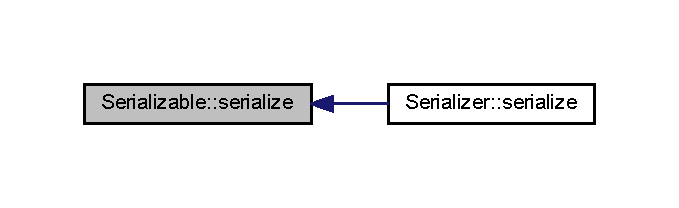
\includegraphics[width=326pt]{class_serializable_aa18caa72dd5e441647f86cc7aab62096_icgraph}
\end{center}
\end{figure}




The documentation for this class was generated from the following file\-:\begin{DoxyCompactItemize}
\item 
Hnefatafl/\hyperlink{_serializable_8hpp}{Serializable.\-hpp}\end{DoxyCompactItemize}

\hypertarget{class_serializer}{\section{Serializer Class Reference}
\label{class_serializer}\index{Serializer@{Serializer}}
}


Static class to serializes a class that inherits \hyperlink{class_serializable}{Serializable}.  




{\ttfamily \#include $<$Serializer.\-hpp$>$}

\subsection*{Static Public Member Functions}
\begin{DoxyCompactItemize}
\item 
static bool \hyperlink{class_serializer_abdb1edae5fe52a2241578bcadae9d265}{serialize} (\hyperlink{class_serializable}{Serializable} $\ast$obj, std\-::string \&output)
\begin{DoxyCompactList}\small\item\em Serializes serializable object. \end{DoxyCompactList}\item 
static bool \hyperlink{class_serializer_a8ee632af50c7ea6a208d3c279b1b39fc}{de\-Serialize} (\hyperlink{class_serializable}{Serializable} $\ast$obj, std\-::string \&input)
\begin{DoxyCompactList}\small\item\em Deserializes serializable object. \end{DoxyCompactList}\end{DoxyCompactItemize}


\subsection{Detailed Description}
Static class to serializes a class that inherits \hyperlink{class_serializable}{Serializable}. 

\begin{DoxyAuthor}{Author}
Rasmus Pettersson Vik 
\end{DoxyAuthor}
\begin{DoxyDate}{Date}
juni 2013 
\end{DoxyDate}


\subsection{Member Function Documentation}
\hypertarget{class_serializer_a8ee632af50c7ea6a208d3c279b1b39fc}{\index{Serializer@{Serializer}!de\-Serialize@{de\-Serialize}}
\index{de\-Serialize@{de\-Serialize}!Serializer@{Serializer}}
\subsubsection[{de\-Serialize}]{\setlength{\rightskip}{0pt plus 5cm}bool Serializer\-::de\-Serialize (
\begin{DoxyParamCaption}
\item[{{\bf Serializable} $\ast$}]{obj, }
\item[{std\-::string \&}]{input}
\end{DoxyParamCaption}
)\hspace{0.3cm}{\ttfamily [static]}}}\label{class_serializer_a8ee632af50c7ea6a208d3c279b1b39fc}


Deserializes serializable object. 


\begin{DoxyParams}[1]{Parameters}
\mbox{\tt in}  & {\em obj} & The object to deserialize \\
\hline
\mbox{\tt in}  & {\em input} & The data to push to the object \\
\hline
\end{DoxyParams}
\begin{DoxyReturn}{Returns}
True on success 
\end{DoxyReturn}


Here is the call graph for this function\-:\nopagebreak
\begin{figure}[H]
\begin{center}
\leavevmode
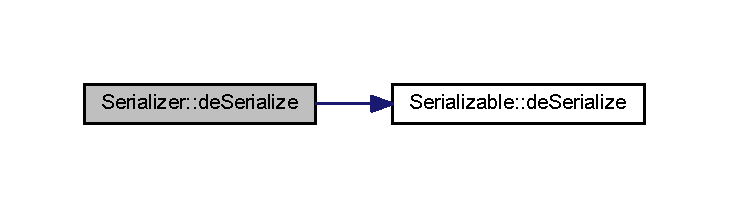
\includegraphics[width=350pt]{class_serializer_a8ee632af50c7ea6a208d3c279b1b39fc_cgraph}
\end{center}
\end{figure}


\hypertarget{class_serializer_abdb1edae5fe52a2241578bcadae9d265}{\index{Serializer@{Serializer}!serialize@{serialize}}
\index{serialize@{serialize}!Serializer@{Serializer}}
\subsubsection[{serialize}]{\setlength{\rightskip}{0pt plus 5cm}bool Serializer\-::serialize (
\begin{DoxyParamCaption}
\item[{{\bf Serializable} $\ast$}]{obj, }
\item[{std\-::string \&}]{output}
\end{DoxyParamCaption}
)\hspace{0.3cm}{\ttfamily [static]}}}\label{class_serializer_abdb1edae5fe52a2241578bcadae9d265}


Serializes serializable object. 


\begin{DoxyParams}[1]{Parameters}
\mbox{\tt in}  & {\em obj} & The object to serialize \\
\hline
\mbox{\tt out}  & {\em output} & Stores the output of the serialization \\
\hline
\end{DoxyParams}
\begin{DoxyReturn}{Returns}
True on success 
\end{DoxyReturn}


Here is the call graph for this function\-:\nopagebreak
\begin{figure}[H]
\begin{center}
\leavevmode
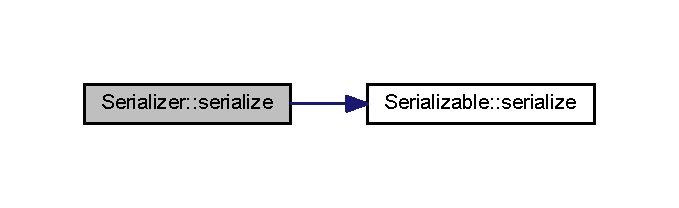
\includegraphics[width=326pt]{class_serializer_abdb1edae5fe52a2241578bcadae9d265_cgraph}
\end{center}
\end{figure}




The documentation for this class was generated from the following files\-:\begin{DoxyCompactItemize}
\item 
Hnefatafl/\hyperlink{_serializer_8hpp}{Serializer.\-hpp}\item 
Hnefatafl/\hyperlink{_serializer_8cpp}{Serializer.\-cpp}\end{DoxyCompactItemize}

\hypertarget{class_tile}{\section{Tile Class Reference}
\label{class_tile}\index{Tile@{Tile}}
}


Describes a tile on the gameboard.  




{\ttfamily \#include $<$Tile.\-hpp$>$}



Inheritance diagram for Tile\-:
\nopagebreak
\begin{figure}[H]
\begin{center}
\leavevmode
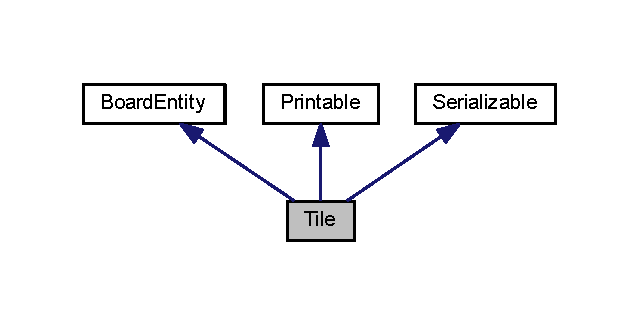
\includegraphics[width=306pt]{class_tile__inherit__graph}
\end{center}
\end{figure}


Collaboration diagram for Tile\-:
\nopagebreak
\begin{figure}[H]
\begin{center}
\leavevmode
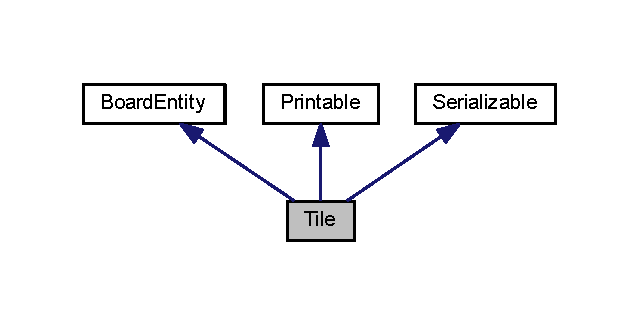
\includegraphics[width=306pt]{class_tile__coll__graph}
\end{center}
\end{figure}
\subsection*{Public Types}
\begin{DoxyCompactItemize}
\item 
enum \hyperlink{class_tile_afa5ef05a7f2ea1f3e44398c001abc738}{Type} \{ {\bfseries E\-M\-P\-T\-Y}, 
{\bfseries C\-O\-R\-N\-E\-R}, 
{\bfseries T\-H\-R\-O\-N\-E}
 \}
\begin{DoxyCompactList}\small\item\em Different types of Tiles. \end{DoxyCompactList}\end{DoxyCompactItemize}
\subsection*{Public Member Functions}
\begin{DoxyCompactItemize}
\item 
\hypertarget{class_tile_a93fdcc8c693044a3bb3590bdb6daed2a}{\hyperlink{class_tile_a93fdcc8c693044a3bb3590bdb6daed2a}{Tile} (void)}\label{class_tile_a93fdcc8c693044a3bb3590bdb6daed2a}

\begin{DoxyCompactList}\small\item\em Default \hyperlink{class_tile}{Tile} Constructor Initialises tile object with Tile\-::\-Type\-::\-E\-M\-P\-T\-Y and position -\/1, -\/1. \end{DoxyCompactList}\item 
\hyperlink{class_tile_a43886ac5f7fbcc05b5c26e34371ec599}{Tile} (const \hyperlink{class_tile}{Tile} \&src)
\begin{DoxyCompactList}\small\item\em \hyperlink{class_tile}{Tile} copy constructor. \end{DoxyCompactList}\item 
\hyperlink{class_tile_ab7a5adaebb9e705923681daf52f1db74}{Tile} (const sf\-::\-Vector2$<$ int $>$ \&pos, const \hyperlink{class_tile_afa5ef05a7f2ea1f3e44398c001abc738}{Tile\-::\-Type} \&\hyperlink{class_tile_af6644c418cbb05f4af1bb0bae756a96f}{type}=Tile\-::\-Type\-::\-E\-M\-P\-T\-Y)
\begin{DoxyCompactList}\small\item\em \hyperlink{class_tile}{Tile} constructor with position and type. \end{DoxyCompactList}\item 
\hypertarget{class_tile_a98634abbd93fa13d0578d7103202d03d}{\hyperlink{class_tile_a98634abbd93fa13d0578d7103202d03d}{$\sim$\-Tile} ()}\label{class_tile_a98634abbd93fa13d0578d7103202d03d}

\begin{DoxyCompactList}\small\item\em \hyperlink{class_tile}{Tile} Destructor. \end{DoxyCompactList}\item 
\hyperlink{class_tile}{Tile} \& \hyperlink{class_tile_a2e2c020a03afc0cdbe98170a05066d9a}{operator=} (const \hyperlink{class_tile}{Tile} \&rhs)
\begin{DoxyCompactList}\small\item\em \hyperlink{class_tile}{Tile} assignment operator. \end{DoxyCompactList}\item 
void \hyperlink{class_tile_af6644c418cbb05f4af1bb0bae756a96f}{type} (const \hyperlink{class_tile_afa5ef05a7f2ea1f3e44398c001abc738}{Tile\-::\-Type} \&type)
\begin{DoxyCompactList}\small\item\em Set the type of the tile. \end{DoxyCompactList}\item 
const \hyperlink{class_tile_afa5ef05a7f2ea1f3e44398c001abc738}{Tile\-::\-Type} \& \hyperlink{class_tile_a816fb8e2d8d48619eccf6e225eca7206}{type} () const 
\begin{DoxyCompactList}\small\item\em Get the type of the tile. \end{DoxyCompactList}\item 
std\-::string \hyperlink{class_tile_acc5f775cb013360f669f5043cbf60cb2}{to\-String} ()
\begin{DoxyCompactList}\small\item\em Gets information about the current tile. \end{DoxyCompactList}\item 
\hypertarget{class_tile_a236311185e4c94d0ceb21bb6d122c4f8}{void \hyperlink{class_tile_a236311185e4c94d0ceb21bb6d122c4f8}{serialize} (Json\-::\-Value \&root)}\label{class_tile_a236311185e4c94d0ceb21bb6d122c4f8}

\begin{DoxyCompactList}\small\item\em Serialize the object to J\-S\-O\-N. \end{DoxyCompactList}\item 
\hypertarget{class_tile_aac6ff96901aa89ac87b1a8385dc6444d}{void \hyperlink{class_tile_aac6ff96901aa89ac87b1a8385dc6444d}{de\-Serialize} (Json\-::\-Value \&root)}\label{class_tile_aac6ff96901aa89ac87b1a8385dc6444d}

\begin{DoxyCompactList}\small\item\em Deserialize the object. \end{DoxyCompactList}\end{DoxyCompactItemize}
\subsection*{Additional Inherited Members}


\subsection{Detailed Description}
Describes a tile on the gameboard. 

\begin{DoxyAuthor}{Author}
Rasmus Pettersson Vik 
\end{DoxyAuthor}
\begin{DoxyDate}{Date}
juni 2013 
\end{DoxyDate}


\subsection{Constructor \& Destructor Documentation}
\hypertarget{class_tile_a43886ac5f7fbcc05b5c26e34371ec599}{\index{Tile@{Tile}!Tile@{Tile}}
\index{Tile@{Tile}!Tile@{Tile}}
\subsubsection[{Tile}]{\setlength{\rightskip}{0pt plus 5cm}Tile\-::\-Tile (
\begin{DoxyParamCaption}
\item[{const {\bf Tile} \&}]{src}
\end{DoxyParamCaption}
)}}\label{class_tile_a43886ac5f7fbcc05b5c26e34371ec599}


\hyperlink{class_tile}{Tile} copy constructor. 


\begin{DoxyParams}[1]{Parameters}
\mbox{\tt in}  & {\em src} & Source to copy from \\
\hline
\end{DoxyParams}


Here is the call graph for this function\-:\nopagebreak
\begin{figure}[H]
\begin{center}
\leavevmode
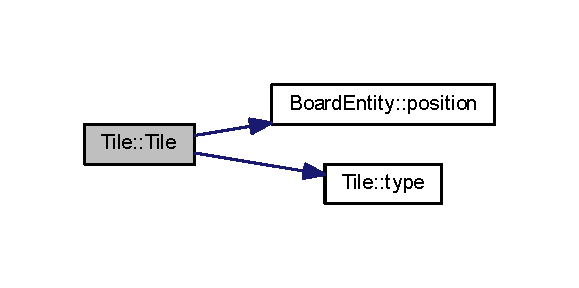
\includegraphics[width=278pt]{class_tile_a43886ac5f7fbcc05b5c26e34371ec599_cgraph}
\end{center}
\end{figure}


\hypertarget{class_tile_ab7a5adaebb9e705923681daf52f1db74}{\index{Tile@{Tile}!Tile@{Tile}}
\index{Tile@{Tile}!Tile@{Tile}}
\subsubsection[{Tile}]{\setlength{\rightskip}{0pt plus 5cm}Tile\-::\-Tile (
\begin{DoxyParamCaption}
\item[{const sf\-::\-Vector2$<$ int $>$ \&}]{pos, }
\item[{const {\bf Tile\-::\-Type} \&}]{type = {\ttfamily Tile\-:\-:Type\-:\-:EMPTY}}
\end{DoxyParamCaption}
)}}\label{class_tile_ab7a5adaebb9e705923681daf52f1db74}


\hyperlink{class_tile}{Tile} constructor with position and type. 

Initializes tile object with the position pos and default type of Tile\-::\-Type\-::\-E\-M\-P\-T\-Y.


\begin{DoxyParams}[1]{Parameters}
\mbox{\tt in}  & {\em pos} & The position to set the tile to. \\
\hline
\mbox{\tt in}  & {\em type} & The type to set the tile to. Default is Tile\-::\-Type\-::\-E\-M\-P\-T\-Y. \\
\hline
\end{DoxyParams}


Here is the call graph for this function\-:\nopagebreak
\begin{figure}[H]
\begin{center}
\leavevmode
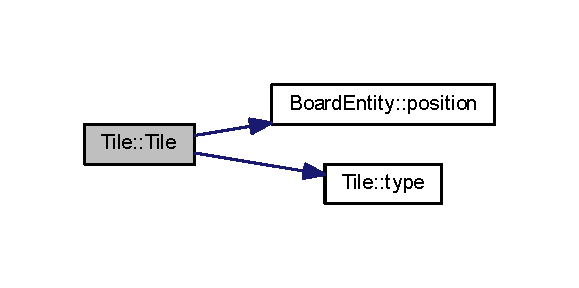
\includegraphics[width=278pt]{class_tile_ab7a5adaebb9e705923681daf52f1db74_cgraph}
\end{center}
\end{figure}




\subsection{Member Function Documentation}
\hypertarget{class_tile_a2e2c020a03afc0cdbe98170a05066d9a}{\index{Tile@{Tile}!operator=@{operator=}}
\index{operator=@{operator=}!Tile@{Tile}}
\subsubsection[{operator=}]{\setlength{\rightskip}{0pt plus 5cm}{\bf Tile} \& Tile\-::operator= (
\begin{DoxyParamCaption}
\item[{const {\bf Tile} \&}]{rhs}
\end{DoxyParamCaption}
)}}\label{class_tile_a2e2c020a03afc0cdbe98170a05066d9a}


\hyperlink{class_tile}{Tile} assignment operator. 


\begin{DoxyParams}[1]{Parameters}
\mbox{\tt in}  & {\em rhs} & Source to copy from \\
\hline
\end{DoxyParams}


Here is the call graph for this function\-:\nopagebreak
\begin{figure}[H]
\begin{center}
\leavevmode
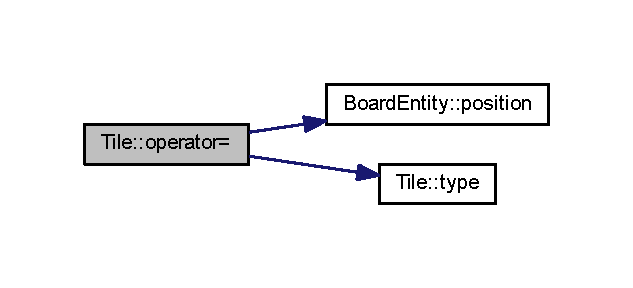
\includegraphics[width=304pt]{class_tile_a2e2c020a03afc0cdbe98170a05066d9a_cgraph}
\end{center}
\end{figure}


\hypertarget{class_tile_acc5f775cb013360f669f5043cbf60cb2}{\index{Tile@{Tile}!to\-String@{to\-String}}
\index{to\-String@{to\-String}!Tile@{Tile}}
\subsubsection[{to\-String}]{\setlength{\rightskip}{0pt plus 5cm}std\-::string Tile\-::to\-String (
\begin{DoxyParamCaption}
{}
\end{DoxyParamCaption}
)\hspace{0.3cm}{\ttfamily [virtual]}}}\label{class_tile_acc5f775cb013360f669f5043cbf60cb2}


Gets information about the current tile. 

\begin{DoxyReturn}{Returns}
Returns the type and position of the tile in a human readable format. 
\end{DoxyReturn}


Implements \hyperlink{class_printable_a489f74384330f76d048d1ccf5c541571}{Printable}.

\hypertarget{class_tile_af6644c418cbb05f4af1bb0bae756a96f}{\index{Tile@{Tile}!type@{type}}
\index{type@{type}!Tile@{Tile}}
\subsubsection[{type}]{\setlength{\rightskip}{0pt plus 5cm}void Tile\-::type (
\begin{DoxyParamCaption}
\item[{const {\bf Tile\-::\-Type} \&}]{type}
\end{DoxyParamCaption}
)}}\label{class_tile_af6644c418cbb05f4af1bb0bae756a96f}


Set the type of the tile. 


\begin{DoxyParams}[1]{Parameters}
\mbox{\tt in}  & {\em type} & The \hyperlink{class_tile_afa5ef05a7f2ea1f3e44398c001abc738}{Tile\-::\-Type} to set. \\
\hline
\end{DoxyParams}


Here is the call graph for this function\-:\nopagebreak
\begin{figure}[H]
\begin{center}
\leavevmode
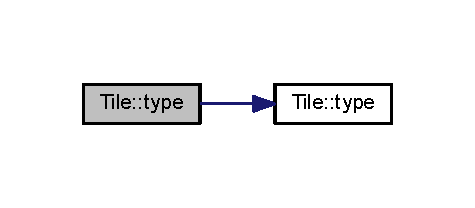
\includegraphics[width=228pt]{class_tile_af6644c418cbb05f4af1bb0bae756a96f_cgraph}
\end{center}
\end{figure}




Here is the caller graph for this function\-:\nopagebreak
\begin{figure}[H]
\begin{center}
\leavevmode
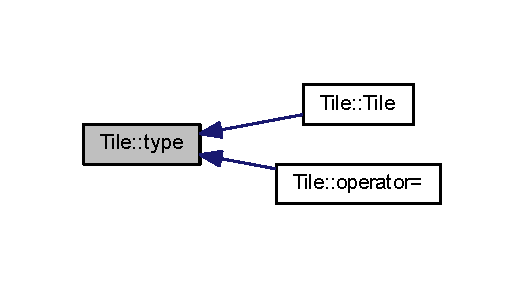
\includegraphics[width=252pt]{class_tile_af6644c418cbb05f4af1bb0bae756a96f_icgraph}
\end{center}
\end{figure}


\hypertarget{class_tile_a816fb8e2d8d48619eccf6e225eca7206}{\index{Tile@{Tile}!type@{type}}
\index{type@{type}!Tile@{Tile}}
\subsubsection[{type}]{\setlength{\rightskip}{0pt plus 5cm}const {\bf Tile\-::\-Type} \& Tile\-::type (
\begin{DoxyParamCaption}
{}
\end{DoxyParamCaption}
) const}}\label{class_tile_a816fb8e2d8d48619eccf6e225eca7206}


Get the type of the tile. 

\begin{DoxyReturn}{Returns}
Returns the type of the tile. 
\end{DoxyReturn}


Here is the caller graph for this function\-:
\nopagebreak
\begin{figure}[H]
\begin{center}
\leavevmode
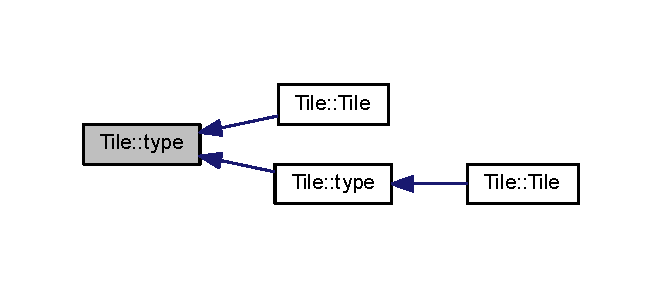
\includegraphics[width=350pt]{class_tile_a816fb8e2d8d48619eccf6e225eca7206_icgraph}
\end{center}
\end{figure}




The documentation for this class was generated from the following files\-:\begin{DoxyCompactItemize}
\item 
Hnefatafl/\hyperlink{_tile_8hpp}{Tile.\-hpp}\item 
Hnefatafl/\hyperlink{_tile_8cpp}{Tile.\-cpp}\end{DoxyCompactItemize}

\chapter{File Documentation}
\hypertarget{_board_8hpp}{\section{Hnefatafl/\-Board.hpp File Reference}
\label{_board_8hpp}\index{Hnefatafl/\-Board.\-hpp@{Hnefatafl/\-Board.\-hpp}}
}
{\ttfamily \#include $<$string$>$}\\*
{\ttfamily \#include $<$vector$>$}\\*
{\ttfamily \#include \char`\"{}Printable.\-hpp\char`\"{}}\\*
{\ttfamily \#include \char`\"{}Tile.\-hpp\char`\"{}}\\*
{\ttfamily \#include \char`\"{}Serializable.\-hpp\char`\"{}}\\*
Include dependency graph for Board.\-hpp\-:
\nopagebreak
\begin{figure}[H]
\begin{center}
\leavevmode
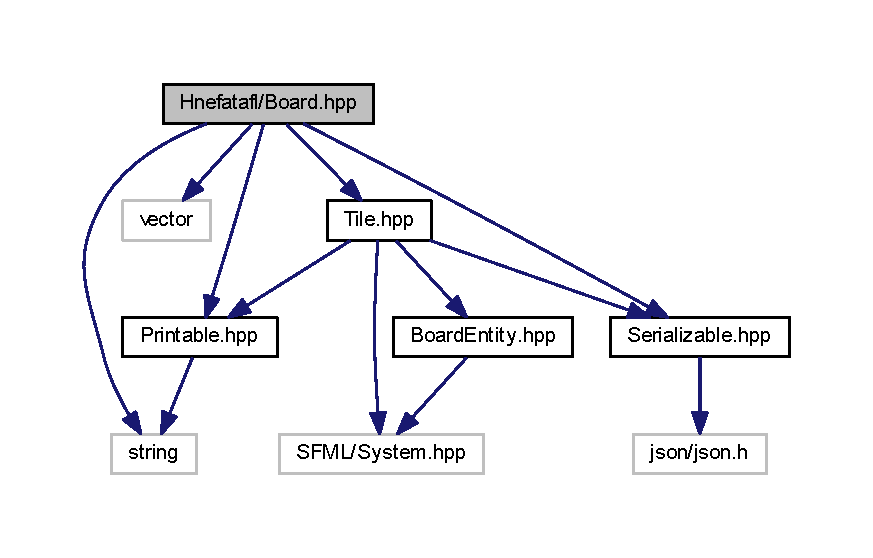
\includegraphics[width=350pt]{_board_8hpp__incl}
\end{center}
\end{figure}
\subsection*{Classes}
\begin{DoxyCompactItemize}
\item 
class \hyperlink{class_board}{Board}
\begin{DoxyCompactList}\small\item\em Defines a board for Hnefatafl. \end{DoxyCompactList}\end{DoxyCompactItemize}


\subsection{Detailed Description}
\begin{DoxyAuthor}{Author}
Rasmus Pettersson Vik 
\end{DoxyAuthor}
\begin{DoxyDate}{Date}
juni 2013
\end{DoxyDate}
Declaration of \hyperlink{class_board}{Board} class 
\hypertarget{_board_entity_8cpp}{\section{Hnefatafl/\-Board\-Entity.cpp File Reference}
\label{_board_entity_8cpp}\index{Hnefatafl/\-Board\-Entity.\-cpp@{Hnefatafl/\-Board\-Entity.\-cpp}}
}
{\ttfamily \#include \char`\"{}Board\-Entity.\-hpp\char`\"{}}\\*
Include dependency graph for Board\-Entity.\-cpp\-:\nopagebreak
\begin{figure}[H]
\begin{center}
\leavevmode
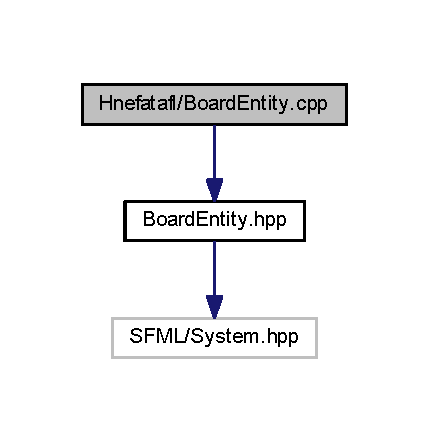
\includegraphics[width=206pt]{_board_entity_8cpp__incl}
\end{center}
\end{figure}


\subsection{Detailed Description}
\begin{DoxyAuthor}{Author}
Rasmus Pettersson Vik 
\end{DoxyAuthor}
\begin{DoxyDate}{Date}
juni 2013
\end{DoxyDate}
Definition of the abstract baseclass \hyperlink{class_board_entity}{Board\-Entity} 
\hypertarget{_board_entity_8hpp}{\section{Hnefatafl/\-Board\-Entity.hpp File Reference}
\label{_board_entity_8hpp}\index{Hnefatafl/\-Board\-Entity.\-hpp@{Hnefatafl/\-Board\-Entity.\-hpp}}
}
{\ttfamily \#include $<$S\-F\-M\-L/\-System.\-hpp$>$}\\*
Include dependency graph for Board\-Entity.\-hpp\-:\nopagebreak
\begin{figure}[H]
\begin{center}
\leavevmode
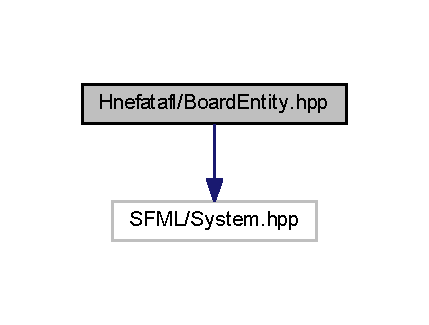
\includegraphics[width=206pt]{_board_entity_8hpp__incl}
\end{center}
\end{figure}
This graph shows which files directly or indirectly include this file\-:
\nopagebreak
\begin{figure}[H]
\begin{center}
\leavevmode
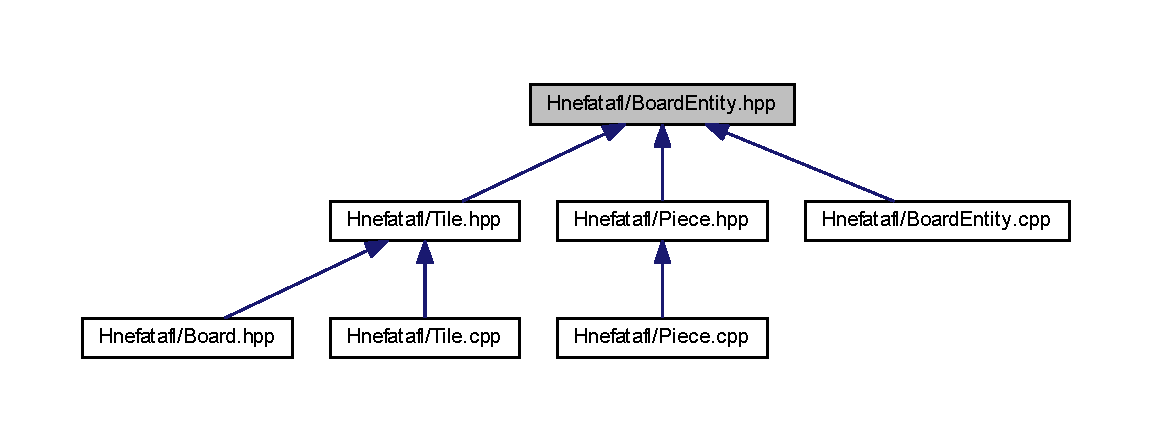
\includegraphics[width=350pt]{_board_entity_8hpp__dep__incl}
\end{center}
\end{figure}
\subsection*{Classes}
\begin{DoxyCompactItemize}
\item 
class \hyperlink{class_board_entity}{Board\-Entity}
\begin{DoxyCompactList}\small\item\em Abstract baseclass for an entity with a position on the gameboard. \end{DoxyCompactList}\end{DoxyCompactItemize}


\subsection{Detailed Description}
\begin{DoxyAuthor}{Author}
Rasmus Pettersson Vik 
\end{DoxyAuthor}
\begin{DoxyDate}{Date}
juni 2013
\end{DoxyDate}
Declaration of the abstract baseclass \hyperlink{class_board_entity}{Board\-Entity} 
\hypertarget{_piece_8cpp}{\section{Hnefatafl/\-Piece.cpp File Reference}
\label{_piece_8cpp}\index{Hnefatafl/\-Piece.\-cpp@{Hnefatafl/\-Piece.\-cpp}}
}
{\ttfamily \#include $<$string$>$}\\*
{\ttfamily \#include $<$sstream$>$}\\*
{\ttfamily \#include \char`\"{}Piece.\-hpp\char`\"{}}\\*
Include dependency graph for Piece.\-cpp\-:\nopagebreak
\begin{figure}[H]
\begin{center}
\leavevmode
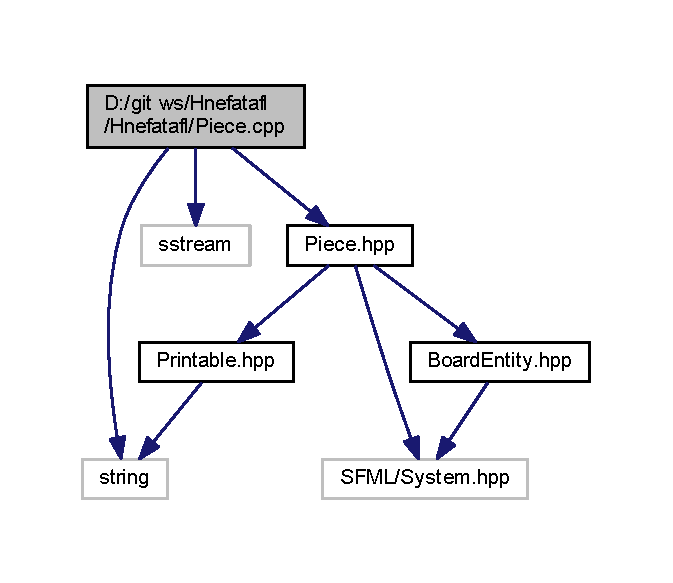
\includegraphics[width=350pt]{_piece_8cpp__incl}
\end{center}
\end{figure}


\subsection{Detailed Description}
\begin{DoxyAuthor}{Author}
Rasmus Pettersson Vik 
\end{DoxyAuthor}
\begin{DoxyDate}{Date}
juni 2013
\end{DoxyDate}
Definition of \hyperlink{class_piece}{Piece} class 
\hypertarget{_piece_8hpp}{\section{Hnefatafl/\-Piece.hpp File Reference}
\label{_piece_8hpp}\index{Hnefatafl/\-Piece.\-hpp@{Hnefatafl/\-Piece.\-hpp}}
}
{\ttfamily \#include $<$S\-F\-M\-L/\-System.\-hpp$>$}\\*
{\ttfamily \#include \char`\"{}Board\-Entity.\-hpp\char`\"{}}\\*
{\ttfamily \#include \char`\"{}Printable.\-hpp\char`\"{}}\\*
{\ttfamily \#include \char`\"{}Serializable.\-hpp\char`\"{}}\\*
Include dependency graph for Piece.\-hpp\-:\nopagebreak
\begin{figure}[H]
\begin{center}
\leavevmode
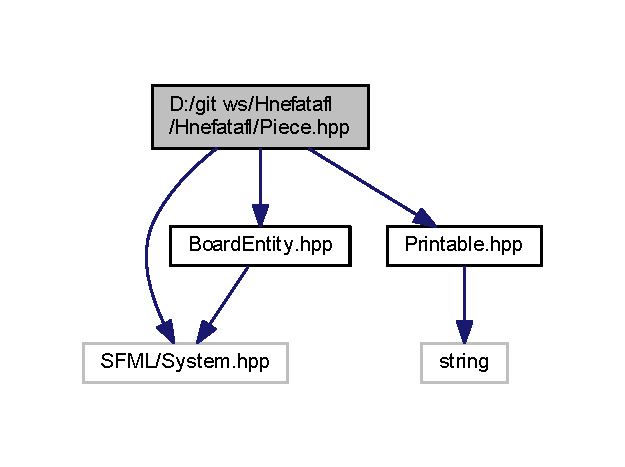
\includegraphics[width=350pt]{_piece_8hpp__incl}
\end{center}
\end{figure}
This graph shows which files directly or indirectly include this file\-:\nopagebreak
\begin{figure}[H]
\begin{center}
\leavevmode
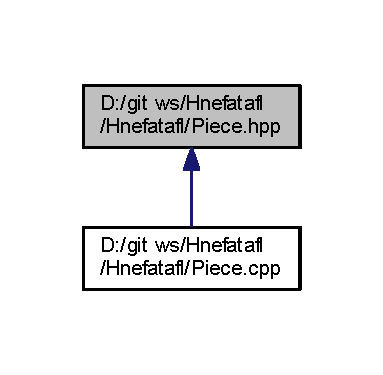
\includegraphics[width=180pt]{_piece_8hpp__dep__incl}
\end{center}
\end{figure}
\subsection*{Classes}
\begin{DoxyCompactItemize}
\item 
class \hyperlink{class_piece}{Piece}
\begin{DoxyCompactList}\small\item\em Describes a piece on the gameboard. \end{DoxyCompactList}\end{DoxyCompactItemize}


\subsection{Detailed Description}
\begin{DoxyAuthor}{Author}
Rasmus Pettersson Vik 
\end{DoxyAuthor}
\begin{DoxyDate}{Date}
juni 2013
\end{DoxyDate}
Declaration of \hyperlink{class_piece}{Piece} class 
\hypertarget{_printable_8hpp}{\section{Hnefatafl/\-Printable.hpp File Reference}
\label{_printable_8hpp}\index{Hnefatafl/\-Printable.\-hpp@{Hnefatafl/\-Printable.\-hpp}}
}
{\ttfamily \#include $<$string$>$}\\*
Include dependency graph for Printable.\-hpp\-:
\nopagebreak
\begin{figure}[H]
\begin{center}
\leavevmode
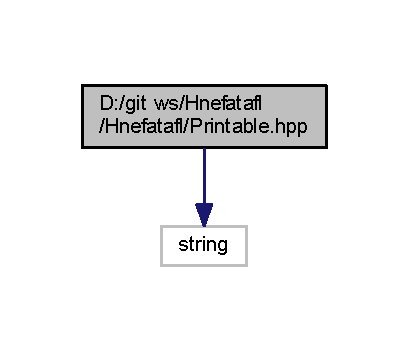
\includegraphics[width=194pt]{_printable_8hpp__incl}
\end{center}
\end{figure}
This graph shows which files directly or indirectly include this file\-:
\nopagebreak
\begin{figure}[H]
\begin{center}
\leavevmode
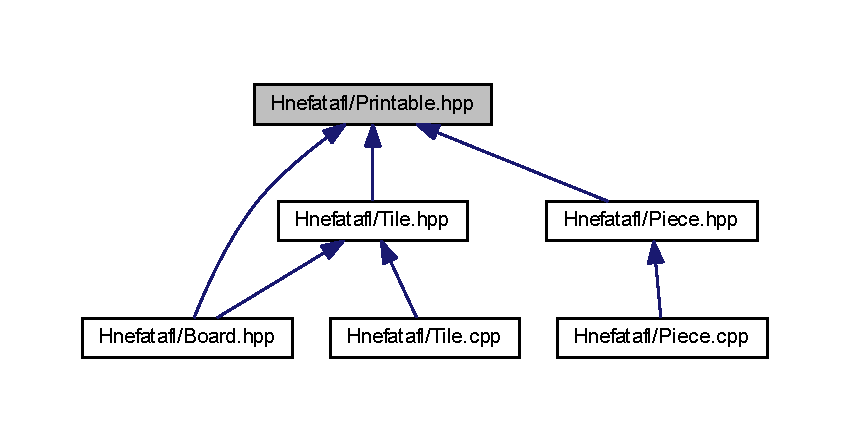
\includegraphics[width=350pt]{_printable_8hpp__dep__incl}
\end{center}
\end{figure}
\subsection*{Classes}
\begin{DoxyCompactItemize}
\item 
class \hyperlink{class_printable}{Printable}
\begin{DoxyCompactList}\small\item\em Abstract class implementing std\-::string \hyperlink{class_printable_a489f74384330f76d048d1ccf5c541571}{to\-String()} functionality. \end{DoxyCompactList}\end{DoxyCompactItemize}


\subsection{Detailed Description}
\begin{DoxyAuthor}{Author}
Rasmus Pettersson Vik 
\end{DoxyAuthor}
\begin{DoxyDate}{Date}
juni 2013
\end{DoxyDate}
Declaration of abstract class. Implements std\-::string to\-String() function 
\hypertarget{_serializable_8hpp}{\section{Hnefatafl/\-Serializable.hpp File Reference}
\label{_serializable_8hpp}\index{Hnefatafl/\-Serializable.\-hpp@{Hnefatafl/\-Serializable.\-hpp}}
}
{\ttfamily \#include $<$json/json.\-h$>$}\\*
Include dependency graph for Serializable.\-hpp\-:
\nopagebreak
\begin{figure}[H]
\begin{center}
\leavevmode
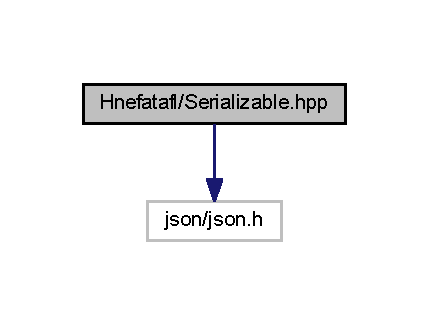
\includegraphics[width=206pt]{_serializable_8hpp__incl}
\end{center}
\end{figure}
This graph shows which files directly or indirectly include this file\-:
\nopagebreak
\begin{figure}[H]
\begin{center}
\leavevmode
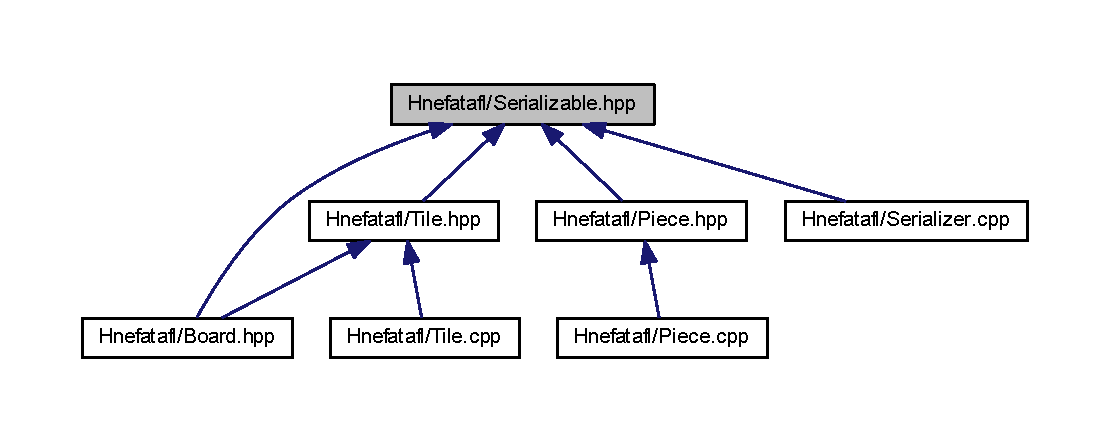
\includegraphics[width=350pt]{_serializable_8hpp__dep__incl}
\end{center}
\end{figure}
\subsection*{Classes}
\begin{DoxyCompactItemize}
\item 
class \hyperlink{class_serializable}{Serializable}
\begin{DoxyCompactList}\small\item\em Interface for serializing classes to J\-S\-O\-N. \end{DoxyCompactList}\end{DoxyCompactItemize}


\subsection{Detailed Description}
\begin{DoxyAuthor}{Author}
Rasmus Pettersson Vik 
\end{DoxyAuthor}
\begin{DoxyDate}{Date}
juni 2013
\end{DoxyDate}
Declaration of virtual baseclass for serializing classes 
\hypertarget{_serializer_8cpp}{\section{Hnefatafl/\-Serializer.cpp File Reference}
\label{_serializer_8cpp}\index{Hnefatafl/\-Serializer.\-cpp@{Hnefatafl/\-Serializer.\-cpp}}
}
{\ttfamily \#include $<$json/json.\-h$>$}\\*
{\ttfamily \#include \char`\"{}Serializer.\-hpp\char`\"{}}\\*
{\ttfamily \#include \char`\"{}Serializable.\-hpp\char`\"{}}\\*
Include dependency graph for Serializer.\-cpp\-:
\nopagebreak
\begin{figure}[H]
\begin{center}
\leavevmode
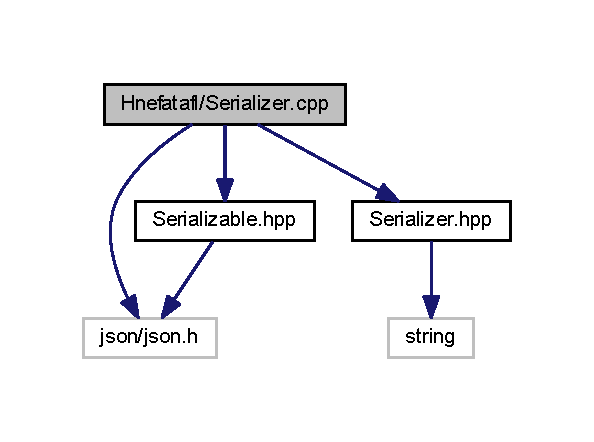
\includegraphics[width=285pt]{_serializer_8cpp__incl}
\end{center}
\end{figure}


\subsection{Detailed Description}
\begin{DoxyAuthor}{Author}
Rasmus Pettersson Vik 
\end{DoxyAuthor}
\begin{DoxyDate}{Date}
juni 2013
\end{DoxyDate}
Definition of serializer class 
\hypertarget{_serializer_8hpp}{\section{Hnefatafl/\-Serializer.hpp File Reference}
\label{_serializer_8hpp}\index{Hnefatafl/\-Serializer.\-hpp@{Hnefatafl/\-Serializer.\-hpp}}
}
{\ttfamily \#include $<$string$>$}\\*
Include dependency graph for Serializer.\-hpp\-:\nopagebreak
\begin{figure}[H]
\begin{center}
\leavevmode
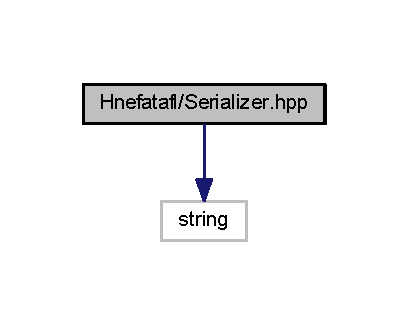
\includegraphics[width=196pt]{_serializer_8hpp__incl}
\end{center}
\end{figure}
This graph shows which files directly or indirectly include this file\-:\nopagebreak
\begin{figure}[H]
\begin{center}
\leavevmode
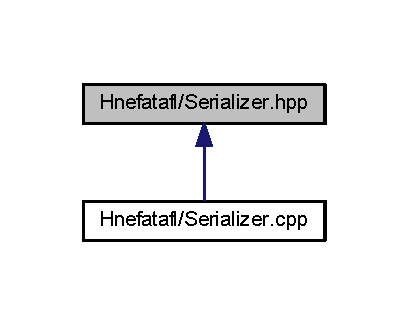
\includegraphics[width=196pt]{_serializer_8hpp__dep__incl}
\end{center}
\end{figure}
\subsection*{Classes}
\begin{DoxyCompactItemize}
\item 
class \hyperlink{class_serializer}{Serializer}
\begin{DoxyCompactList}\small\item\em Static class to serializes a class that inherits \hyperlink{class_serializable}{Serializable}. \end{DoxyCompactList}\end{DoxyCompactItemize}


\subsection{Detailed Description}
\begin{DoxyAuthor}{Author}
Rasmus Pettersson Vik 
\end{DoxyAuthor}
\begin{DoxyDate}{Date}
juni 2013
\end{DoxyDate}
Declaration of \hyperlink{class_serializer}{Serializer} class 
\hypertarget{_tile_8cpp}{\section{D\-:/git ws/\-Hnefatafl/\-Hnefatafl/\-Tile.cpp File Reference}
\label{_tile_8cpp}\index{D\-:/git ws/\-Hnefatafl/\-Hnefatafl/\-Tile.\-cpp@{D\-:/git ws/\-Hnefatafl/\-Hnefatafl/\-Tile.\-cpp}}
}
{\ttfamily \#include $<$sstream$>$}\\*
{\ttfamily \#include \char`\"{}Tile.\-hpp\char`\"{}}\\*
Include dependency graph for Tile.\-cpp\-:\nopagebreak
\begin{figure}[H]
\begin{center}
\leavevmode
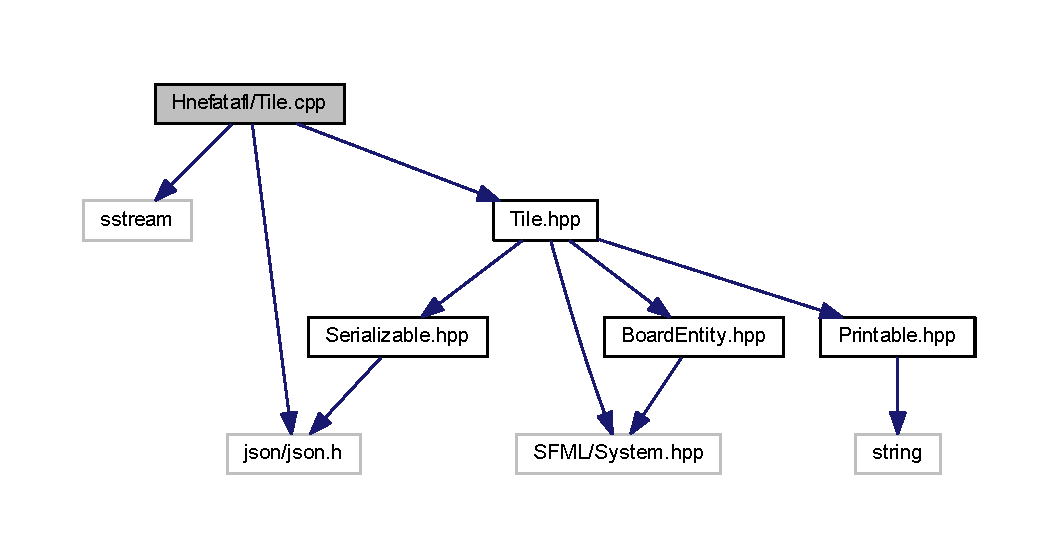
\includegraphics[width=310pt]{_tile_8cpp__incl}
\end{center}
\end{figure}


\subsection{Detailed Description}
\begin{DoxyAuthor}{Author}
Rasmus Pettersson Vik 
\end{DoxyAuthor}
\begin{DoxyDate}{Date}
juni 2013
\end{DoxyDate}
Definition of the \hyperlink{class_tile}{Tile} class-\/ 
\hypertarget{_tile_8hpp}{\section{D\-:/git ws/\-Hnefatafl/\-Hnefatafl/\-Tile.hpp File Reference}
\label{_tile_8hpp}\index{D\-:/git ws/\-Hnefatafl/\-Hnefatafl/\-Tile.\-hpp@{D\-:/git ws/\-Hnefatafl/\-Hnefatafl/\-Tile.\-hpp}}
}
{\ttfamily \#include $<$S\-F\-M\-L/\-System.\-hpp$>$}\\*
{\ttfamily \#include \char`\"{}Board\-Entity.\-hpp\char`\"{}}\\*
{\ttfamily \#include \char`\"{}Printable.\-hpp\char`\"{}}\\*
Include dependency graph for Tile.\-hpp\-:\nopagebreak
\begin{figure}[H]
\begin{center}
\leavevmode
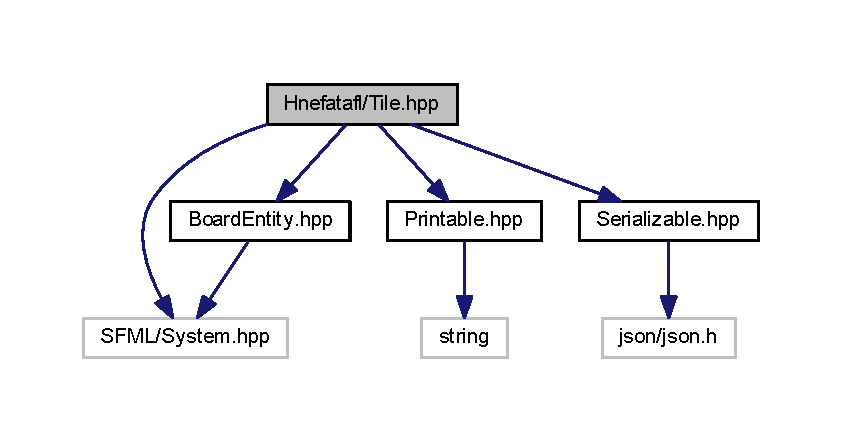
\includegraphics[width=300pt]{_tile_8hpp__incl}
\end{center}
\end{figure}
This graph shows which files directly or indirectly include this file\-:\nopagebreak
\begin{figure}[H]
\begin{center}
\leavevmode
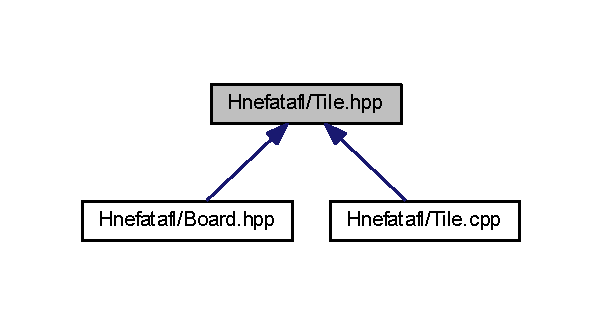
\includegraphics[width=174pt]{_tile_8hpp__dep__incl}
\end{center}
\end{figure}
\subsection*{Classes}
\begin{DoxyCompactItemize}
\item 
class \hyperlink{class_tile}{Tile}
\begin{DoxyCompactList}\small\item\em Describes a tile on the gameboard. \end{DoxyCompactList}\end{DoxyCompactItemize}


\subsection{Detailed Description}
\begin{DoxyAuthor}{Author}
Rasmus Pettersson Vik 
\end{DoxyAuthor}
\begin{DoxyDate}{Date}
juni 2013
\end{DoxyDate}
Declaration of \hyperlink{class_tile}{Tile} class 
\addcontentsline{toc}{part}{Index}
\printindex
\end{document}
